% ------ | ------- | ------- | ------- | ------- | ------- | ------- | ------- |
%
\documentclass[twocolumn,twoside,fleqn,12pt]{article}
%
% This lightly writes DRAFT across each page.
\usepackage{draftcopy}
%
% Handling footnotes
\usepackage{ftnright}                  % Places footnotes in right column
\setlength{\skip\footins}{8pt}         % Sets footnote size to 8pt
\addtolength{\textheight}{1in}         % Adjusts spacing for footnotes
\preparefootins                        % Saves these parameters
%
% For handling encapsulated postscript files.
\usepackage[pdftex]{graphicx}
%\usepackage{epsfig}
%
% Single column figure
%\begin{figure}
%   \centering
%   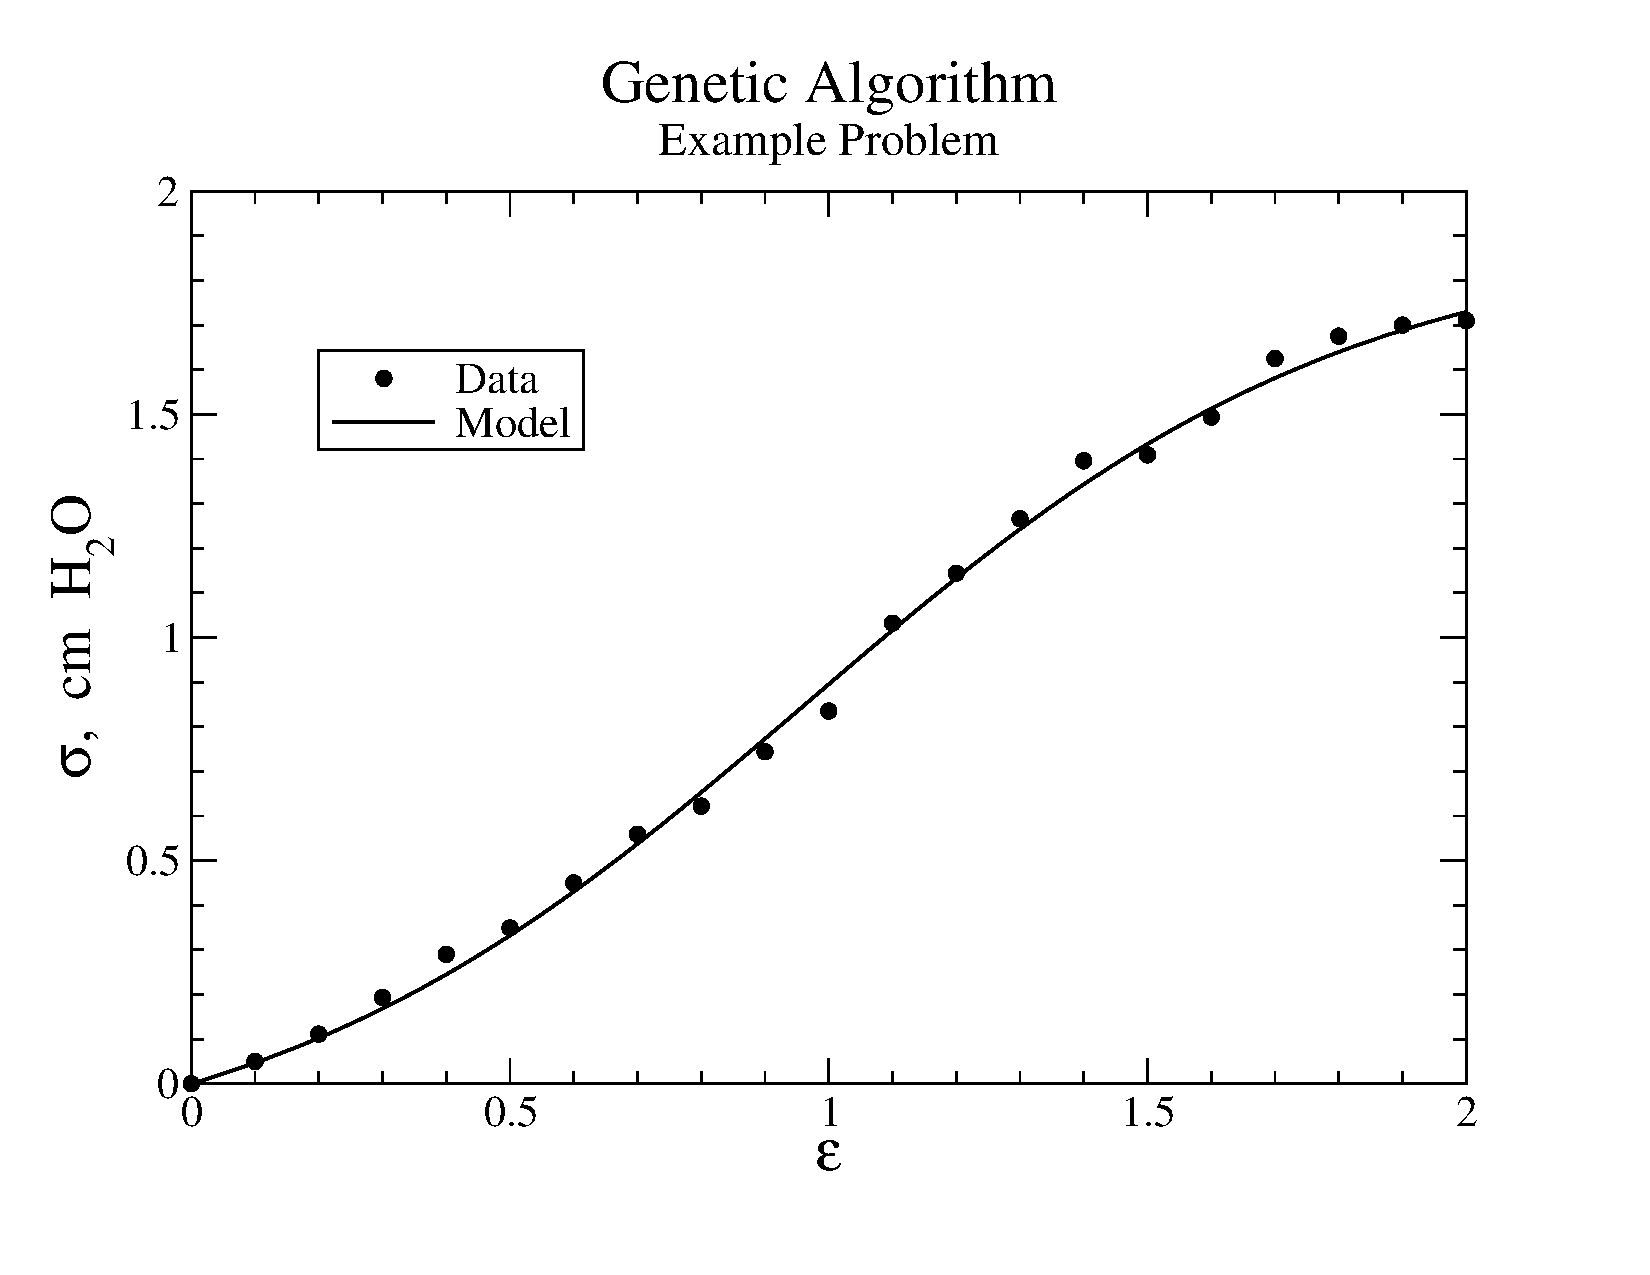
\includegraphics[angle=-90,width=8cm]{gaExample.pdf}
%   \caption{...}
%   \label{...}
%\end{figure}
%
% Double column figure
%\begin{figure*}
%   {\par\centering
%   \resizebox*{1.0\textwidth}{.25\textheight}
%   {\includegraphics[angle=-90]{<figure.eps>}}
%   \par}
%   \caption{\label{<figureLabel>}%
%   }
%\end{figure*}
%
% Tables are the same. A one column table has the structure
%\begin{table}
%  ...
%\end{table}
%
% while a two-column table is created with
%\begin{table*}
%  ...
%\end{table*}
%
%
% Set up babel for typesetting bibliographies.
\usepackage[english]{babel}  %language selection
\selectlanguage{english}
% Languages supported by babel include:
%   american, austrian, brazil, catalan, croatian, czech, danish, dutch,
%   english, esperanto, finnish, french, galician, german, italian, magyar,
%   norsk, nynorsk, polish, portuges, romanian, russian, slovak, slovene,
%   spanish, swedish, turkish.
%
% Select the default text font which is used, for example,
% in the typesetting of the front matter of a paper
% and in the typesetting text in formulae, e.g., sin.
% The Monotype Baskerville fonts are sold separately at: http://www.fonts.com.
%\renewcommand{\rmdefault}{cmr}        % computer modern roman
%\renewcommand{\rmdefault}{txr}        % TX fonts
%\renewcommand{\rmdefault}{ptm}        % Adobe times roman
%\renewcommand{\rmdefault}{mbv}        % Baskerville with inline numbers
\renewcommand{\rmdefault}{mbvj}        % Baskerville with old-style numbers
%
% If AMS-LaTeX macros are to used, load them before mtpro.
% MTPro will replace the AMS fonts, but not its macros.
\usepackage{amsmath, amsthm}
%
% Load MathTime Professional II fonts - commercial fonts
% For sales and other information visit www.pctex.com.
% The following math fonts are created:
%   \mathrm   \mathit    \mathsf   \mathtt
%   \mathbf   \mathbold  \mbf      \mathbb
%   \mathcal  \mathbcal  \mathscr  \mathbscr  \mathfrak
%\usepackage[subscriptcorrection,slantedGreek,boldalphabet,mtpccal,mtpscr,mtpfrak,mtphrb,zswash,nofontinfo]{mtpro2}
\usepackage[subscriptcorrection,slantedGreek,mtpccal,mtpscr,mtpfrak,mtphrb,zswash,nofontinfo]{mtpro2}
%
% Introduce the text fonts.
%
% Define a set of macros for characterizing text fonts.
%   medium fonts   roman     san serif    typewriter
%     upright     \fontrm    \fontss      \fonttt
%     slant       \fontsl    \fontsssl    \fontttsl
%     small cap   \fontsc    \fontsssc    \fontttsc
%     italic      \fontit
%
%   bold fonts     roman     san serif    typewriter
%     upright     \boldrm    \boldss      \boldtt
%     slant       \boldsl    \boldsssl    \boldttsl
%     small cap   \boldsc    \boldsssc    \boldttsc
%     italic      \boldit
%
% Establish the default font encoding scheme to use.
\DeclareFontEncoding{T1}{}{}           % specify text font encoding scheme
\DeclareFontEncoding{TS1}{}{}          % specify text companion font encoding
%
% Normal text fonts.
\DeclareFontFamily{T1}{txr}{\hyphenchar\font=127}
\DeclareFontShape{T1}{txr}{m}{n}{<-> t1xr}{}
\DeclareFontShape{T1}{txr}{m}{sl}{<-> t1xsl}{}
\DeclareFontShape{T1}{txr}{m}{sc}{<-> t1xsc}{}
\DeclareFontShape{T1}{txr}{m}{it}{<-> t1xi}{}
\renewcommand{\normalfont}{\usefont{T1}{txr}{m}{n}}
\newcommand{\fontrm}[1]{\normalfont{#1}}
\newcommand{\fontsl}[1]{\usefont{T1}{txr}{m}{sl}{#1}\normalfont}
\newcommand{\fontsc}[1]{\usefont{T1}{txr}{m}{sc}{#1}\normalfont}
\newcommand{\fontit}[1]{\usefont{T1}{txr}{m}{it}{#1}\normalfont}
%
% Bold text fonts.
\DeclareFontFamily{T1}{txb}{\hyphenchar\font=127}
\DeclareFontShape{T1}{txb}{bx}{n}{<-> t1xb}{}
\DeclareFontShape{T1}{txb}{bx}{sl}{<-> t1xbsl}{}
\DeclareFontShape{T1}{txb}{bx}{sc}{<-> t1xbsc}{}
\DeclareFontShape{T1}{txb}{bx}{it}{<-> t1xbi}{}
\newcommand{\boldrm}[1]{\usefont{T1}{txb}{bx}{n}{#1}\normalfont}
\newcommand{\boldsl}[1]{\usefont{T1}{txb}{bx}{sl}{#1}\normalfont}
\newcommand{\boldsc}[1]{\usefont{T1}{txb}{bx}{sc}{#1}\normalfont}
\newcommand{\boldit}[1]{\usefont{T1}{txb}{bx}{it}{#1}\normalfont}
%
% Normal san serif fonts.
\DeclareFontFamily{T1}{txss}{\hyphenchar\font=127}
\DeclareFontShape{T1}{txss}{m}{n}{<-> s * [0.95] t1xss}{}
\DeclareFontShape{T1}{txss}{m}{sl}{<-> s * [0.95] t1xsssl}{}
\DeclareFontShape{T1}{txss}{m}{sc}{<-> s * [0.95] t1xsssc}{}
\newcommand{\fontss}[1]{\usefont{T1}{txss}{m}{n}{#1}\normalfont}
\newcommand{\fontsssl}[1]{\usefont{T1}{txss}{m}{sl}{#1}\normalfont}
\newcommand{\fontsssc}[1]{\usefont{T1}{txss}{m}{sc}{#1}\normalfont}
%
% Bold san serif fonts.
\DeclareFontFamily{T1}{txssb}{\hyphenchar\font=127}
\DeclareFontShape{T1}{txssb}{bx}{n}{<-> s * [0.95] t1xbss}{}
\DeclareFontShape{T1}{txssb}{bx}{sl}{<-> s * [0.95] t1xbsssl}{}
\DeclareFontShape{T1}{txssb}{bx}{sc}{<-> s * [0.95] t1xbsssc}{}
\newcommand{\boldss}[1]{\usefont{T1}{txssb}{bx}{n}{#1}\normalfont}
\newcommand{\boldsssl}[1]{\usefont{T1}{txssb}{bx}{sl}{#1}\normalfont}
\newcommand{\boldsssc}[1]{\usefont{T1}{txssb}{bx}{sc}{#1}\normalfont}
%
% Normal typewriter fonts.
\DeclareFontFamily{T1}{txtt}{\hyphenchar\font=127}
\DeclareFontShape{T1}{txtt}{m}{n}{<-> t1xtt}{}
\DeclareFontShape{T1}{txtt}{m}{sl}{<-> t1xttsl}{}
\DeclareFontShape{T1}{txtt}{m}{sc}{<-> t1xttsc}{}
\newcommand{\fonttt}[1]{\usefont{T1}{txtt}{m}{n}{#1}\normalfont}
\newcommand{\fontttsl}[1]{\usefont{T1}{txtt}{m}{sl}{#1}\normalfont}
\newcommand{\fontttsc}[1]{\usefont{T1}{txtt}{m}{sc}{#1}\normalfont}
%
% Bold typewriter fonts.
\DeclareFontFamily{T1}{txttb}{\hyphenchar\font=127}
\DeclareFontShape{T1}{txttb}{bx}{n}{<-> t1xbtt}{}
\DeclareFontShape{T1}{txttb}{bx}{sl}{<-> t1xbttsl}{}
\DeclareFontShape{T1}{txttb}{bx}{sc}{<-> t1xbttsc}{}
\newcommand{\boldtt}[1]{\usefont{T1}{txttb}{bx}{n}{#1}\normalfont}
\newcommand{\boldttsl}[1]{\usefont{T1}{txttb}{bx}{sl}{#1}\normalfont}
\newcommand{\boldttsc}[1]{\usefont{T1}{txttb}{bx}{sc}{#1}\normalfont}
%
\usepackage{xspace} % provides appropriate spacing
% Redefine the standard text font selecting macros.
\renewcommand{\textrm}[1]{\fontrm{#1}\xspace}
\renewcommand{\textbf}[1]{\boldrm{#1}\xspace}
\renewcommand{\textit}[1]{\fontit{#1}\xspace}
\renewcommand{\textsc}[1]{\fontsc{#1}\xspace}
\renewcommand{\textsf}[1]{\fontss{#1}\xspace}
\renewcommand{\textsl}[1]{\fontsl{#1}\xspace}
\renewcommand{\texttt}[1]{\fonttt{#1}\xspace}
\renewcommand{\textup}[1]{\fontrm{#1}\xspace}
% If xspace provides unwanted spacing, do not use the
% base \font## or \bold## commands instead of \text##.
%
\newcommand{\eg}{e.g.,\xspace}
\newcommand{\ie}{i.e.,\xspace}
\newcommand{\viz}{viz.,\xspace}
\newcommand{\cf}{cf.\@\xspace}
\newcommand{\eq}{Eq.\@\xspace}
\newcommand{\eqs}{Eqs.\@\xspace}
\newcommand{\etc}{etc.\@\xspace}
\newcommand{\fig}{Fig.\@\xspace}
\newcommand{\figs}{Figs.\@\xspace}
\newcommand{\vs}{vs.\@\xspace}
%
% For underlining options
%\usepackage{ulem}
%    \uline{important}   underlined text
%    \uuline{urgent}     double-underlined text
%    \uwave{boat}        wavy underline
%    \sout{wrong}        line drawn through word
%    \xout{removed}      marked over with //////
%
% Define macros for writing tensor equations.
%
% Macro for typesetting numbers in text.
\newcommand{\scalar}[1]%
   {\fontencoding{TS1}\selectfont #1\fontencoding{T1}\selectfont}
%
% Macros for typesetting vectors - italic roman.
\DeclareMathAlphabet{\mathitbb}{U}{mt2hrb}{m}{it}
\newcommand{\vecFld}[1]{\ensuremath{\mathbold{#1}}}
\newcommand{\vecEle}[1]{\ensuremath{\mathit{#1}}}
\newcommand{\vecMtx}[1]{\ensuremath{\mathitbb{#1}}}
%
% Macros for typesetting tensors of second rank - upright roman.
\newcommand{\tenFld}[1]{\ensuremath{\mbf{#1}}}
\newcommand{\tenEle}[1]{\ensuremath{\mathrm{#1}}}
\newcommand{\tenMtx}[1]{\ensuremath{\mathbb{#1}}}
%
% Macros for typesetting tensors of fourth rank - italic san serif.
\DeclareMathAlphabet{\mathsfbb}{U}{mt2bb}{m}{it}
\newcommand{\TenFld}[1]{\ensuremath{\text{\boldsssl{#1}}}}
\newcommand{\TenEle}[1]{\ensuremath{\text{\fontsssl{#1}}}}
\newcommand{\TenMtx}[1]{\ensuremath{\mathsfbb{#1}}}
%
% Macros for typesetting greek symboled fields.
\newcommand{\grkFld}[1]{\ensuremath{\mathbold{#1}}}
\newcommand{\grkEle}[1]{\ensuremath{#1}}
\newcommand{\grkMtx}[1]{\ensuremath{\mathitbb{#1}}}
%
% Macros for creating nice text and script fractions.
%   There is a cleaner way to do this; for example,
%   \newcommand*{\textfrac}[2]{%
%      {\fontfamily{<fontname>1}\selectfont #1}%
%      \textfractionsolidus
%      {\fontfamily{<fontname>0}\selectfont #2}}%
%   See http://www.ctan.org/tex-archive/macros/latex/doc/fntguide.pdf
%   Sec. V.5: Using the feature of expert fonts
%   Here we must use the following hack because Adobe Times Roman and
%   Baskerville expert fonts do not contain the superior <fontname>1
%   and inferior <fontname>0 glyphs in their font tables.
% Do not break these long lines into multiple lines
% Spaces CANNOT be present - they cause unwanted `rubber' spacing
\newcommand{\textfrac}[2]
   {\leavevmode
    \kern.05em\raise.6ex\hbox{\ensuremath{\scriptstyle{#1}}}\kern-.05em\hspace{0em}/\hspace{0em}\kern-.05em\lower.2ex\hbox{\ensuremath{\scriptstyle{#2}}}\kern.05em
   }
\newcommand{\scriptfrac}[2]
   {\leavevmode
    \kern.05em\raise.3ex\hbox{\ensuremath{\scriptscriptstyle{#1}}}\kern-.05em\hspace{0em}\hbox{\ensuremath{\scriptstyle{/}}}\hspace{0em}\kern-.05em\lower.25ex\hbox{\ensuremath{\scriptscriptstyle{#2}}}\kern.05em
   }
%
% Layout and formatting of the document.
%
% Macro used for creating nomenclatures, etc.
\newcommand{\namelistlabel}[1]{\mbox{#1}\hfil}
\newenvironment{namelist}[1]
   {\begin{list}{}%
      {\let\makelabel\namelistlabel%
       \settowidth{\labelwidth}{#1}%
       \setlength{\leftmargin}{1.1\labelwidth}%
       \setlength{\itemsep}{-6pt}%
      }%
   }{\end{list}%
}
%
% page size
\pdfpagewidth 8.5in
\pdfpageheight 11in
% top margin
\setlength\topmargin{-0.25in}
% header properties
\setlength\headheight{0in}
\setlength\headsep{0in}
% printed size on paper
\setlength\textheight{9.5in}
\setlength\textwidth{7in}
% margins for two-sided printing
\setlength\oddsidemargin{0in}
\setlength\evensidemargin{-0.4in}
% paragraph properties
\setlength\parindent{0.25in}
\setlength\parskip{0.05in}
% Column separation
\setlength{\columnsep}{15pt}
\setlength{\columnseprule}{0pt}
% Fill page
\flushbottom
%
%
% don't hyphenate so much - default = 200, max (never hyphenate) = 10,000
\hyphenpenalty=800
%
% two column float page must be 90% full
\renewcommand\dblfloatpagefraction{.90}
% two column top float can cover up to 80% of page
\renewcommand\dbltopfraction{.80}
% float page must be 90% full
\renewcommand\floatpagefraction{.90}
% top float can cover up to 80% of page
\renewcommand\topfraction{.80}
% bottom float can cover up to 80% of page
\renewcommand\bottomfraction{.80}
% at least 10% of a normal page must contain text
\renewcommand\textfraction{.1}
%
% separation between floats and text
\setlength\dbltextfloatsep{9pt plus 5pt minus 3pt }
% separation between two column floats and text
\setlength\textfloatsep{10pt plus 4pt minus 3pt}
%
%
% Additional declarations beyond my standard template.
%
%%%%%%%%%%%%%%%%%%%%%%%%%%%%%%%%%%%%%%%%%%%%%%%%%%
%
%
%
\begin{document}
%
\bibliographystyle{asme}       % numeric bibliography format
%\bibliographystyle{plain}
%
\title{\textsf{BEL}\\
       A \textsf{.NET} Computational Package Written in Zonnon\\
       Part I of the Users Guide\\
       \phantom{A}}
%
\author{Alan D.\ Freed\\
\and
\mbox{}\hfill Clifford H.\ Spicer Chair in Engineering\\
\mbox{}\hfill College of Science, Engineering \& Technology\\
\mbox{}\hfill Saginaw Valley State University\\
\mbox{}\hfill 202 Pioneer Hall, 7400 Bay Road\\
\mbox{}\hfill University Center, MI 48710\\
\mbox{}\hfill E-Mail: \texttt{adfreed@svsu.edu}\\
}
%
\date{\today}



\maketitle
\normalfont


\begin{figure}
   \centering
   
\includegraphics[width=8cm]{BelLogo.pdf}
\end{figure}

\begin{abstract}
This document describes the core set of modules belonging to the
\textsf{BEL} software library written in \textsf{Zonnon} for the
\textsf{.NET} and \textsf{Mono} frameworks.  \textsf{BEL} provides
a simple, computational, programming interface for the purpose of
assisting in rapid program development (especially in the area of
computational continuum mechanics) by leveraging the wide diversity
of existing \textsf{.NET} and \textsf{Mono} libraries with the simple
logical constructs of the \textsf{Zonnon} programming language.
\textsf{BEL}'s interfaces for its core modules are cataloged in the
appendices.
\end{abstract}


\section{Introduction}
\label{introSection}

\textsf{BEL} is an acronym taken for my research laboratory: The Biological
Engineering Laboratory at Saginaw Valley State University. What \textsf{BEL}
is and what it provides are quite different from what one might expect,
given this affiliation. \textsf{BEL} arose out of the author's desire to
interface with the \textsf{.NET} and \textsf{Mono} Frameworks for the purpose
of writing computational software programs in the \textsf{Zonnon} programming
language \cite{Zonnon09,Zonnon10}.

\textsf{Zonnon} is the most recent descendant from the family
tree \textsf{Euler}\slash \textsf{Algol}\slash \textsf{Pascal}\slash
\textsf{Modula}\slash \textsf{Oberon} of programming languages
developed by Profs.\ \textsc{Niklaus Wirth} and \textsc{J\"urg Gutknecht}
from the Computer Systems Institute at ETH Zurich (Eidgen\"ossische
Technische Hochschule, Zentrum, \ie the Swiss Federal Institute of
Technology, Zurich).  \textsf{Zonnon} was created specifically for
\textsf{.NET}, with compiler versions available for both the \textsf{.NET}
and \textsf{Mono} Frameworks. Sponsored by Xamarin, Mono is an open 
source implementation of Microsoft's .NET Framework based on the 
ECMA standards for C\# and the Common Language Runtime.
The \textsf{Zonnon} compiler targets the \textsf{.NET} 
Framework~2.0.

The \textsf{Zonnon} compiler, documentation, example programs, 
and even \textsf{BEL} itself, are free to download
from \texttt{http:\slash\slash www.zonnon.ethz.ch}.
The home page for Microsoft's \textsf{.NET} Framework is at
\texttt{http:\slash\slash www.microsoft.com\slash net}.
\textsf{Mono}'s is at
\texttt{http:\slash\slash www.mono-project.com\slash Main_Page}.


\subsection{Licensing}

Licensing of the \textsf{BEL} library, both its software and
documentation, is addressed in the \textit{Licensing of the
Software and its Documentation\/} part to this user guide.


\subsubsection{NPlot}

\textsf{NPlot} is the \textsf{.NET} graphics engine used by 
\textsf{BEL} for creating plots.  The \textsf{NPlot} home page is:  
\texttt{http://netcontrols.org/nplot/wiki/}.  \textsf{NPlot} 
is released under the terms of a 3-clause-BSD license.  Specifically: 
\begin{quote}
   ``NPlot---A charting library for .NET. \\
   Copyright \copyright\ 2003-2006 Matt Howlett and others.
   All rights reserved.  
   
   Redistribution and use in source and binary forms, with or 
   without modification, are permitted provided that the following
   conditions are met:
   \begin{enumerate}
   \item Redistributions of source code must retain the above 
         copyright notice, this list of conditions and the 
         following disclaimer.
   \item Redistributions in binary form must reproduce the 
         above copyright notice, this list of conditions and the 
         following disclaimer in the documentation and/or other 
         materials provided with the distribution.   
   \item Neither the name of NPlot nor the names of its contributors 
        may be used to endorse or promote products derived from this
        software without specific prior written permission.
   \end{enumerate}
   THIS SOFTWARE IS PROVIDED BY THE COPYRIGHT HOLDERS AND CONTRIBUTORS 
   "AS IS" AND ANY EXPRESS OR IMPLIED WARRANTIES, INCLUDING, BUT NOT 
   LIMITED TO, THE IMPLIED WARRANTIES OF MERCHANTABILITY AND FITNESS 
   FOR A PARTICULAR PURPOSE ARE DISCLAIMED. IN NO EVENT SHALL THE 
   COPYRIGHT OWNER OR CONTRIBUTORS BE LIABLE FOR ANY DIRECT, INDIRECT,
   INCIDENTAL, SPECIAL, EXEMPLARY, OR CONSEQUENTIAL DAMAGES (INCLUDING, 
   BUT NOT LIMITED TO, PROCUREMENT OF SUBSTITUTE GOODS OR SERVICES; 
   LOSS OF USE, DATA, OR PROFITS; OR BUSINESS INTERRUPTION) HOWEVER 
   CAUSED AND ON ANY THEORY OF LIABILITY, WHETHER IN CONTRACT, STRICT
   LIABILITY, OR TORT (INCLUDING NEGLIGENCE OR OTHERWISE) ARISING IN 
   ANY WAY OUT OF THE USE OF THIS SOFTWARE, EVEN IF ADVISED OF THE 
   POSSIBILITY OF SUCH DAMAGE.''
\end{quote}

\subsection{Version}

This document corresponds to software version 4.2 of \textsf{BEL}, \today.
\textsf{Zonnon} and \textsf{NPlot} target the \textsf{.NET} Framework~2. 
The version number is exported from module \textsf{Bel.Version} 
as the string variable \texttt{version}.


\subsection{Required Libraries}

Two external libraries are required to compile \textsf{BEL}; 
they are: \textsf{System.Drawing.dll} and \textsf{NPlot.dll}. 
\textsf{NPlot} has different libraries for \textsf{.NET} and 
\textsf{mono}, because \textsf{System.Drawing.Drawing2D} is 
not implemented in the \textsf{mono} framework.


\subsection{Known Issues}

None


\subsection{Feedback}

I consider this to be a living document. If there is some aspect that is
wanting, or if you have corrections and/or additions that you believe
would benefit other users of \textsf{BEL}, please forward them to 
\texttt{adfreed@svsu.edu}.


\section{Design Philosophy}
%\phantomsection
\label{designSection}

The original motivation behind my writing \textsf{BEL} was a need to economize
on the number of numeric types available so as to avoid an explosion in
the number of extended higher-level types to be created.  Recent changes
in the language\slash compiler have drastically reduced the potential
for type explosion.  Consequently, major changes were introduced into
\vs 4.0 from it predecessors.  \textsf{BEL} is now more a collection
of libraries than it is a miniature framework.  \textsf{BEL} is now
leaner.  The author continues to be guided by \fontsc{Wirth}'s design
paradigm: \textbf{Seek simplicity!}

A conscious design decision was to use \textsl{value\/} (or
static) types as wrappers around \textsl{ref\/} (or dynamic pointer)
types whenever possible. There are applications where this is not
desirable, \eg nodes in data structures lend themselves nicely to
pointer types so that linkages can be created, broken and recreated,
as needed, without the need to move their data in memory. For most
computational needs, however, static types seem to work best, so as
to avoid unwanted side effects. Yet, data structures like arrays and
matrices are most useful when their structures are dynamically created.
\textsf{BEL} tries to balance the best of both these worlds by appearing
to the user as a collection of static types, while hiding and managing
their dynamic data structures internally.  The nuisance of creating
dynamic types, to the extent that is possible, has been removed from
the user and relegated to the \textsf{BEL} system.

The core set of modules that define \textsf{BEL} include input\slash
output (IO), a graphing capability, a set of array\slash matrix types,
and basic data structures.

The definition modules for various types exported by \textsf{BEL} are given
in App.\ \ref{defnAppendix}. The software interfaces to the core modules
of \textsf{BEL} are provided in App.\ \ref{ioAppendix}--\ref{dataAppendix}.


\section{Input\slash Output}
\label{coreSection}

There are a great number of \textsf{.NET} modules that deal with file IO.
The author has economized on three file types: log, data, and text files;
and two graphic types: curves and plots.  All files created are
written into the subdirectory \texttt{<executable>/iofiles} right below
where your program's executable file resides. \textsf{BEL} will automatically
create the \texttt{iofiles} directory if it does not already exist.

\subsection{Log File}

\textsf{Zonnon} does not have a construct for throwing a runtime exception,
so a logging capability was created where messages can be written that
could prove useful to a programmer who is trying to debug their code.
This log file is written into file \texttt{<executable>/iofiles/logFile.txt}.
If a log file already exists, the old file will be copied to
\texttt{last_logFile.txt}, and a new file \texttt{logFile.txt}
will then be opened. If there was an existing old log file,
it will be deleted before your prior log file is renamed to
\texttt{last_logFile.txt}.

This log file is automatically created when module \texttt{Bel.Log}
is first loaded into memory. There are three procedures that a programmer
may call: \texttt{Message, WarningMessage}, and \texttt{ErrorMessage}.
A \texttt{Message} writes a string into the log file, while a
\texttt{WarningMessage} or an \texttt{ErrorMessage} writes predefined
messages into the file, and a string that locates where the message
was issued. The scripts for predefined messages reside in module
\texttt{Bel.Log} and are listed in App.~\ref{logAppendix}.
The difference between a warning and an error message is that runtime \
execution continues whenever a warning is issued; whereas, the program
terminates immediately after an error message has been logged to file.

The last line in each executable file that you write should be the
command that closes the log file, \ie \texttt{Bel.Log.Close}.


\subsection{Data Files}

Data files are used to write\slash read data to\slash from a file on
your hard disk in binary format.
They are encoded in UTF-16 unicode format.
A writer created with \texttt{Bel.DataFiles.OpenWriter} takes a
file name as a string and returns a \textsf{.NET} framework writer of
type \texttt{System.IO.BinaryWriter}. The file name that you supply will
be stripped of any path information and\slash or extension you gave it.
It will be given the file extension \texttt{.dat} and placed under the
directory \texttt{<executable>/iofiles} along side the log file.  When
you are done writing to the file, close it by calling the procedure
\texttt{CloseWriter}.
The corresponding \texttt{OpenReader} and \texttt{CloseReader} procedures
are to be called  when it is time to read in data from a file.

The \textsf{.NET} binary reader and writer objects that are supplied by these
procedures are, in fact, the arguments to be sent to the \texttt{Load}
and \texttt{Store} methods that utilizer's of the \texttt{Bel.Object} 
definition must implement.


\subsection{Text Files}

Text files mirror data files in all aspects, except that these files are
human-readable text files instead of machine-readable binary files.
They are encoded in UTF-16 unicode format and given a \texttt{.txt}
extension.  \textbf{Note}: if you try to view one of these files in 
an editor that does not support full unicode, then it will look like 
it is a binary file.

The programmer has more control over how a text file looks or 
is constructed, versus a binary data file, via the various 
methods that belong to the \textsf{.NET} classes of
\texttt{System.IO.StreamWriter} and \texttt{System.IO.StreamReader},
instances of which are supplied by the \texttt{Bel.TextFiles} procedures
\texttt{OpenWriter} and \texttt{OpenReader}.  The methods belonging to
these \textsf{.NET} classes can be found on their documentation web pages.


\subsection{2D Graphical Curves}

Three enumerated types exist to aid in specializing any given
data set in a graph; they are: \texttt{Color}, \texttt{Dimension}, 
and \texttt{Marker}.  Type \texttt{Color} can have one of nine values:
\texttt{black}, \texttt{blue}, \texttt{gray}, \texttt{green},
\texttt{orange}, \texttt{pink}, \texttt{purple}, \texttt{red}, 
and \texttt{yellow}.  Type \texttt{Dimension} can have one of 
five values: \texttt{tiny}, \texttt{small}, \texttt{medium}, 
\texttt{large}, and \texttt{huge}.  And type \texttt{Marker} 
can have one of eleven values: \texttt{circle}, \texttt{cross},
\texttt{diamond}, \texttt{flagDown}, \texttt{flagUp}, \texttt{none},
\texttt{plus}, \texttt{square}, \texttt{triangle}, 
\texttt{triangleDown}, and \texttt{triangleUp}.  

Instances of type\texttt{Bel.Curves.Attributes} provide the 
characteristics that belong to a given curve in a plot.  
Attributes \texttt{color}, \texttt{dimension}, and \texttt{mark} 
belong to the enumerations \texttt{Color}, \texttt{Dimension}, 
and \texttt{Marker}.  Specifying the string variable
\texttt{label} provides the name of the curve as it is to 
appear in the legend.  Markers \texttt{circle}, \texttt{square}, 
and \texttt{triangle} can be filled (\texttt{filled} = 
\boldttsl{true}) or unfilled (\texttt{filled} = \boldttsl{false}), 
as can the vertical bars in a histogram.  These bars can either 
be centered at their associated $x$ value (\texttt{centered} 
= \boldttsl{true}) or not (\texttt{centered} = \boldttsl{false}), 
as can the horizontal steps in a step plot.  Procedure 
\texttt{Initialize} sets: \texttt{centered} $\leftarrow$ 
\boldttsl{true}, \texttt{color} $\leftarrow$ \texttt{black}, 
\texttt{dimension} $\leftarrow$ \texttt{medium}, 
\texttt{filled} $\leftarrow$ \boldttsl{false}, 
\texttt{label} to the empty string, and \texttt{mark} 
$\leftarrow$ \texttt{none}.

Two types of data sets are considered for plotting.  Both contain the 
\texttt{Bel.Curves.Attributes} data in field \texttt{attributes}. 
Instances of the type \texttt{Bel.Curves.DataY} provide the ordinate 
($y$) values, with the abscissa ($x$) values being assigned 
sequential values of 1, 2, 3, $\ldots$, assigned by the row position 
of their ordinates.  Procedure \texttt{Assign} converts 
\textsf{Zonnon} arrays into \textsf{.NET} arrays that 
\textsf{NPlot} understands and can use, and assigns them 
to the variable \texttt{data}.  Likewise, instances of type 
\texttt{Bel.Curves.DataXY} provide the ordinate ($y$) 
and abscissa ($x$) values to be plotted.  Procedures 
\texttt{AssignX} and \texttt{AssignY} convert \textsf{Zonnon} 
arrays into \textsf{.NET} arrays that \textsf{NPlot} understands 
and can use, and assigns them to the \texttt{xData} and 
\texttt{yData} variables.  Procedure \texttt{Initialize} 
initializes the attributes and sets the data vectors to 
\boldttsl{nil } for both types.

Six procedures are provided in module \texttt{Bel.Curves} 
for constructing various curves for plots.  \texttt{LineCurveY} 
and \texttt{LineCurveXY} produce line curves, accepting data 
belonging to \texttt{DataY} and \texttt{DataXY}, respectively. 
\texttt{PointCurveY} and \texttt{PointCurveXY} produce point 
curves, accepting data belonging to \texttt{DataY} and 
\texttt{DataXY}, respectively.  And \text{StepCurve} produces 
a step curve for data belonging to type \texttt{DataY}. 
These five functions have a like fingerprint.  They accept 
a data set describing the curve and they return an instance 
of the associated curve as an \textsf{NPlot} object.  The 
sixth procedure has a different interface; it is for plotting 
histograms.  Procedure \texttt{Histogram} accepts two inputs: 
\texttt{histogramData} is an instance of \texttt{DataY} whose 
attributes describe the appearance of the histogram, while 
\texttt{normalCurve} is an instance of \texttt{Attributes} 
describing how the bell curve is to be drawn.  Procedure 
\texttt{Histogram} provides five outputs: \texttt{mean}, 
\texttt{median}, and \texttt{stdDev} provide the sample mean, 
median, and sample standard deviation of the data in the 
histogram, which are also used in constructing the bell curve,
while variables \texttt{histogram} and \texttt{normalPlot} 
provide \textsf{NPlot} objects for the histogram and bell-curve 
to be drawn in a plot.

Noticeably missing is the ability to draw dashed and dotted curves. 
This capability requires library \texttt{System.Drawing.Drawing2D}, 
which is not part of the \textsf{mono} distribution of \textsf{.NET}. 
Consequently, this feature is not included here so that \textsf{BEL} 
can be used in both the \textsf{.NET} and \textsf{mono} frameworks.


\subsection{2D Graphical Plots}

\textsf{NPlot} is the underlying graphics engine that is used in 
\texttt{Bel.Plots}.  After one has created a collection of 
curves of types \texttt{NPlot.LinePlot}, \texttt{NPlot.PointPlot}, 
\texttt{NPlot.StepPlot}, and\slash or \texttt{NPlot.HistogramPlot}, 
which are supplied by the various procedures of \texttt{Bel.Curves}, 
one can create a \texttt{Bel.Plots.Plot}.  Type \texttt{Plot}
has ten methods to help you create your figures.

\texttt{Bel.Plots.Plot.Create} supplies the blank canvas upon which
your graph will be drawn.  It has two argument, the width and height 
of your graph in \texttt{pixels}.  500 pixels for the width and 400
pixels for the height were assigned in the test code.
(The outputs shown in Figs.~\ref{imageFig} \& \ref{histoFig} 
have been scaled by \LaTeX.)

\begin{figure}
   \centering
   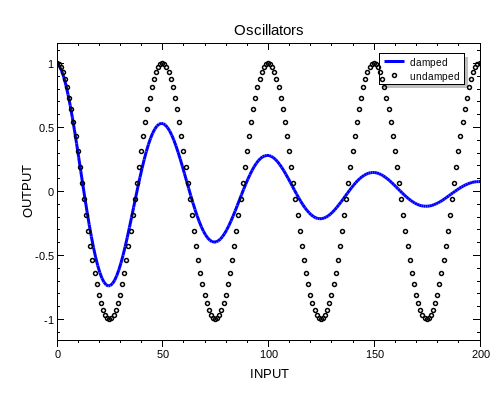
\includegraphics[width=8cm]{testPlot.png}
   \caption{Graph created by the software distributed in the
      \mbox{\texttt{testPlot}} directory in \mbox{\textsf{BEL}}'s
      distribution folder.}
   \label{imageFig}
\end{figure}

\begin{figure}
   \centering
   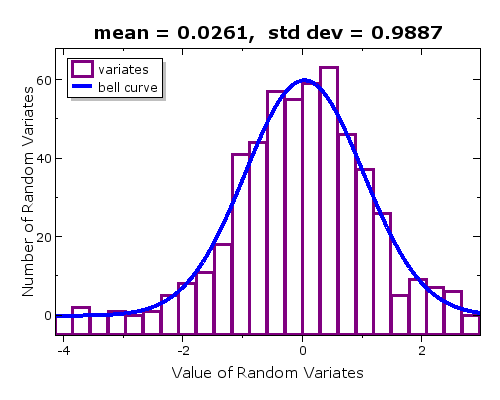
\includegraphics[width=8cm]{histogram.png}
   \caption{Graph created by the software distributed in the
      \mbox{\texttt{testPlot}} directory in \mbox{\textsf{BEL}}'s
      distribution folder.}
   \label{histoFig}
\end{figure}

\texttt{Bel.Plots.Plot.AddAxes} writes axes unto the graph.
Automatic scaling is turned on and, at present, cannot be turned off.
There are four arguments for this procedure.  The first two are
\boldttsl{boolean } valued switches.  When \boldttsl{true } they
make their respective axis logarithmic; otherwise, 
that axis will be taken to be linear.  The
last two are \boldttsl{string\/}s that assign a label to each axis.
The first argument of each pairing is for the x-axis, while the second
is for the y-axis.

\texttt{Bel.Plots.Plot.AddLegend} is the procedure that will write a legend
onto your graph.  It can be placed at one of the four inside corners of
the plot, positioned according to the passed value of enumeration type
\texttt{Location} which can have values: \texttt{lowerLeft}, 
\texttt{lowerRight}, \texttt{upperLeft} and \texttt{upperRight},
the latter two being shown in Figs.~\ref{imageFig} \& \ref{histoFig}, 
or it can be placed outside the plot to the upper-right by passing 
\texttt{Location.outside}.  A legend will 
be displayed only if this command is called.

\texttt{Bel.Plots.Plot.AddTitle} writes a title above the graph.
It is passed as a \boldttsl{string } argument.

\texttt{Bel.Plots.Plot.AddLineCurve} draws a line curve on the
plot's canvas.  These curves are supplied by either 
\texttt{Bel.Curves.LineCurveY} or \texttt{Bel.Curves.LineCurveXY}. 
Line curves are drawn as straight segmented lines.  

\texttt{Bel.Plots.Plot.AddPointCurve} draws a point curve on the
plot's canvas.  These curves are supplied by either
\texttt{Bel.Curves.PointCurveY} or \texttt{Bel.Curves.PointCurveXY}.  

\texttt{Bel.Plots.Plot.AddStepCurve} draws a step curve on the 
plot's canvas.  This curve type is supplied by 
\texttt{Bel.Curves.StepCurve}.

\texttt{Bel.Plots.Plot.AddHistogram} draws a histogram on the 
plot's canvas.  This curve type is supplied by 
\texttt{Bel.Curves.Histogram}.

The order in which curves are attached to a plot is the order that 
they are displayed in the legend.

\texttt{Bel.Plots.Plot.AddText} writes a string passed as \texttt{text} 
to the plot positioned \texttt{atX} and \texttt{atY}, which hold 
world coordinate values, i.e., coordinates that align with those of 
the x- and y-axes.

\textbf{Note}: You must call \texttt{AddAxes} before adding 
any curves to the plot via
\texttt{AddLineCurve}, \texttt{AddPointCurve}, \texttt{AddStepCurve}, 
or \texttt{AddHistogram}.  You must call \texttt{AddText} after the 
curves have been added to the plot.

A call to \texttt{Bel.Plots.Plot.Save} will write your finished graph to
a bitmap file given the name that you supplied.  It will have a
\texttt{.bmp} extension, and will be written into the \texttt{iofiles}
subdirectory below where your executable file resides, in standard
\textsf{BEL} manner.

\textsf{NPlot} has many capabilities that are not utilized in \textsf{BEL}.  
Some of these enhancements are expected to be adopted in future releases.


\section{Numeric Types}

Module \texttt{Bel.Types} exports six numeric constants; they are: 
\texttt{MaximumInteger} is the largest possible value of type 
\boldttsl{integer}, \texttt{Epsilon} is machine epsilon, 
\texttt{MaximumReal} is the largest possible value of type 
\boldttsl{real } that retains full precision in its digits, 
\texttt{MinimumReal} is the smallest positive value of type 
\boldttsl{real } that retains full precision in its digits, 
\texttt{NaN} represents not a number, \texttt{NegativeInfinity} 
handles values less than -\texttt{MaximumReal} while 
\texttt{PositiveInfinity} handles values greater than 
\texttt{MaximumReal}.\footnote{
  \texttt{Epsilon}, \texttt{MaxValue}, and \texttt{MinValue} exported 
  by \texttt{System.Double} are distinct from \textsf{BEL}'s 
  constants \texttt{Epsilon}, \texttt{MaximumReal}, 
  and \texttt{MinimumReal}.
}

Module \texttt{Bel.Types} provides a number of definitions for a variety of
array and matrix types; specifically: \texttt{Boolean\-Vector, Integer\-Vector,
Real\-Vector;} and \texttt{Boolean\-Matrix, Integer\-Matrix, Real\-Matrix};
all of which have \textsl{math\/} attributes.  The syntax of these additional
operations mimics that of the popular \textsf{MatLab}\footnote{
   \textsf{MatLab} is a powerful but pricy mathematical programming
   environment that is marketed by MathWorks 
   \texttt{www.mathworks.com/products/matlab}.
} 
development environment; specifically, assignments can be made much
more simply via
\begin{namelist}{matrix}
\item[array] $\mathbf{x} := [ x_1 , x_2 , \dots , x_n ]$
\item[matrix] $\mathbf{A} := [[ A_{11} , A_{12} , \dots , A_{1n} ],$\\
              \phantom{$\mathbf{A} := [$}$
                              [ A_{21} , A_{22} , \dots , A_{2n} ],$\\
              \phantom{$\mathbf{A} := [$} \vdots \\
              \phantom{$\mathbf{A} := [$}$
                              [ A_{m1} , A_{m2} , \dots , A_{mn} ]]$
\end{namelist}
Element-wise operations include:
\begin{namelist}{binary}
\item[unary] ``$-$''    \hspace{2em} negation \\
             ``$\sim$'' \hspace{2em} inversion
\item[binary] ``$.*$''  \hspace{2em} multiply \\
              ``$./$''  \hspace{2em} division \\
              ``$.\!<$''  \hspace{1.5em} less than \\
              ``$.\!<=$'' \hspace{0.75em} less than or equal \\
              ``$.\!>$''  \hspace{1.5em} greater than \\
              ``$.\!>=$'' \hspace{0.75em} greater than or equal \\
              ``$.\!=$''  \hspace{1.5em} equal \\
              ``$.\#$'' \hspace{1.8em} not equal
\end{namelist}
Array and matrix operations include:
\begin{namelist}{binary}
\item[unary] ``!''      \hspace{1.4em} transpose
\item[binary] ``$+$''   \hspace{1em} addition \\
              ``$-$''   \hspace{1.1em} subtraction \\
              ``$*$''   \hspace{1.25em} multiplication via index contraction \\
              ``$\slash$'' \hspace{1.4em} right division \\
              \mbox{}\hspace{0.75cm} \texttt{X := B/A} solves
                  $\mathbf{X} \cdot \mathbf{A} = \mathbf{B}$ for $\mathbf{X}$\\
              \mbox{}\hspace{0.75cm} \texttt{x := b/A} solves
                  $\mathbf{x}^T \mathbf{A} = \mathbf{b}$ for $\mathbf{x}$\\
              ``$\backslash$'' \hspace{1.4em} left division \\
              \mbox{}\hspace{0.75cm} \texttt{X := A$\backslash$B} solves
                  $\mathbf{A} \cdot \mathbf{X} = \mathbf{B}$ for $\mathbf{X}$\\
              \mbox{}\hspace{0.75cm} \texttt{x := A$\backslash$b} solves
                  $\mathbf{A} \mathbf{x} = \mathbf{b}$ for $\mathbf{x}$
\end{namelist}
Math arrays and matrices have other operators\slash functions
that can be used by them, but the above are the most common and
useful.

This module provides a variety of useful procedures. \texttt{IsFinite,
IsInfinite}, and \texttt{IsNaN} provide tests that check the value
held by a \textsl{real}.  Procedures \texttt{BooleanToString,
IntegerToString}, \texttt{NumberToString}, and \texttt{RealToString} 
print out the values held by their arguments.  \texttt{NumberToString}
prints out reals in decimal notation, while \texttt{RealToString} 
prints out reals in scientific notation, both being able to be 
written to a specified number of significant digits.  To parse
these fields, one can call procedures \texttt{StringToBoolean,
StringToInteger}, and \texttt{StringToReal}.

For writing the base \textsf{Zonnon} types to file, one can use the
\texttt{Bel.Types} procedures \texttt{Store\-String,}
\texttt{Store\-Boolean,} \texttt{Store\-Integer,} \texttt{Store\-Real,}
\texttt{Store\-Boolean\-Vector,} \texttt{Store\-Integer\-Vector,}
\texttt{Store\-Real\-Vector,}
\texttt{Store\-Boolean\-Matrix,} \texttt{Store\-Integer\-Matrix}, and
\texttt{Store\-Real\-Matrix}, which can in turn be read from file via
their counterpart procedures \texttt{Load\-String,} \texttt{Load\-Boolean,}
\texttt{Load\-Integer,} \texttt{Load\-Real,} \texttt{Load\-Boolean\-Vector,}
\texttt{Load\-Integer\-Vector,} \texttt{Load\-Real\-Vector,}
\texttt{Load\-Boolean\-Matrix,}
\texttt{Load\-Integer\-Matrix}, and \texttt{Load\-Real\-Matrix}.


\subsection{Series}

\texttt{Bel.Series} exports three kinds of series that are
either infinite series summed to some convergence criteria, or that are
truncated series. These are: continued fractions, power series, and
rational power series. A continued fraction has the form
\begin{displaymath}
   y = b_0(x) + \frac{a_1 (x)}{b_1(x) +
             \frac{a_2(x)}{b_2(x) +
             \frac{a_3(x)}{b_3(x) + \cdots}}} 
\end{displaymath}
where coefficients $a_i(x)$ and $b_i(x)$ can be functions of $x$.  
In contrast, a truncated continued fraction has the form
\begin{displaymath}
   y = b_0 + \frac{a_1 x}{b_1 +
             \frac{a_2 x}{b_2 +
             \frac{a_3 x}{\cdots + 
             \frac{a_{n-1} x}{b_{n-1} + 
             \frac{a_n x}{b_n}}}}} 
\end{displaymath}
where here the coefficients $a_i$ and $b_i$ are constants.
A power series has the form
\begin{displaymath}
   y = a_0 + a_1 x + a_2 x^2 + a_3 x^3 + \cdots ,
\end{displaymath}
while a rational power series has the form
\begin{displaymath}
   y = \frac{a_0 + a_1 x + a_2 x^2 + a_3 x^3 + \cdots}
       {b_0 + b_1 x + b_2 x^2 + b_3 x^3 + \cdots} 
\end{displaymath}
wherein $a_i$ and $b_i$ are constants.
These kinds of series are often used to define or approximate mathematical
functions in computer applications \cite{Hartetal68}.

The procedures that compute a series to convergence require the user to
write instances of procedure type \texttt{Bel.Series.GetCoef},
which in turn is to be passed
to the procedures in this module so that a series' coefficients can be
determined.  Such a function will have three arguments.  The first sends
an integer that specifies the index for which the coefficient is to be
returned.  The second sends the argument of the function being evaluated.
And the third is updated by the procedure; it being a boolean flag to
force termination of a summation prior to convergence (\eg when it is taking
too long). Such a procedure returns a coefficient for the series, \eg $a_2$.


\subsection{Math}

Module \texttt{Bel.Math} exports two, fundamental, mathematical constants;
they being: $\mathtt{E} = \mathrm{e}^1 = \mathrm{e}$ = \scalar{2.71828182845905}
and $\mathtt{PI} = \pi$ = \scalar{3.14159265358979}, when expressed to
machine accuracy. \texttt{Math} also exports the more common math
functions that one will likely have need of:

\medskip
\noindent\texttt{Random} returns a random number in [0,1].

\noindent\texttt{Max} returns the greater of its two arguments.

\noindent\texttt{Min} returns the lesser of its two arguments.

\noindent\texttt{Ceiling} returns the smallest integer value that is greater
than or equal to its argument.

\noindent\texttt{Floor} returns the greatest integer value that is less than
or equal to its argument.

\noindent\texttt{Round} returns the integer value that is closest to its
argument.

\noindent\texttt{Abs} returns the absolute value of its argument.

\noindent\texttt{Sign} returns one if its argument is greater than zero,
minus one if its argument is less than zero, and zero if it is zero.

\noindent\texttt{Sqrt} returns the square root of its argument.

\noindent\texttt{Power} returns the first argument, $x$, raised to the power
of the second argument, $y$, \viz $x^y$.

\noindent\texttt{Pythag} returns the Euclidean distance between two
numbers, \ie $\sqrt{x^2 + y^2}$.

\noindent\texttt{Log} returns the base 10 logarithm of its argument.

\noindent\texttt{Ln} returns the natural logarithm of its argument.

\noindent\texttt{Exp} returns the exponential of its argument.

\noindent\texttt{Sin} returns the sine of its argument.

\noindent\texttt{Cos} returns the cosine of its argument.

\noindent\texttt{Tan} returns the tangent of its argument.

\noindent\texttt{ArcSin} returns the inverse sine of its argument.

\noindent\texttt{ArcCos} returns the inverse cosine of its argument.

\noindent\texttt{ArcTan} returns the inverse tangent of its argument.

\noindent\texttt{ArcTan2} returns the quadrant-correct inverse tangent of its
two arguments, \ie $\tan^{-1}(y/x)$, where rise $y$ is its first argument,
and run $x$ is its second.

\noindent\texttt{Sinh} returns the hyperbolic sine of its argument.

\noindent\texttt{Cosh} returns the hyperbolic cosine of its argument.

\noindent\texttt{Tanh} returns the hyperbolic tangent of its argument.

\noindent\texttt{ArcSinh} returns the inverse hyperbolic sine of its argument.

\noindent\texttt{ArcCosh} returns the inverse hyperbolic cosine of its argument.

\noindent\texttt{ArcTanh} returns the inverse hyperbolic tangent of its
argument.



\section{Definitions}

A \textsf{Zonnon} \textbf{definition} is a contractual interface that all
who implement it must obey.  One definition can \textbf{refine} another, 
but not in a circular manner.  \textsf{Zonnon} uses a compositional 
inheritance model based on aggregation \cite{Zonnon10}.


\subsection{Entity}

A \texttt{Bel.Entity} is the base definition for all \textsf{Zonnon} objects
that are to be created within the \textsf{BEL} framework. Any implementation of
\texttt{Bel.Entity} is required to export two methods.  \texttt{Initialize}
is called to prepare an object for use. \texttt{Nullify} is called after
an object is no longer needed. Its purpose is for setting all dynamically
allocated internal variables to \texttt{nil}, when they exist, so that they
can be collected later by the garbage collector of the \textsf{.NET}
and \textsf{Mono} frameworks.


\subsection{Object}

\texttt{Bel.Object} is a persistent \texttt{Bel.Entity};
in other words, implementations of interface \texttt{Bel.Object} can be
saved to a file for later retrieval and use.  \texttt{Bel.Object}
\textsf{refines} the \texttt{Bel.Entity} definition.  In addition
to the two methods required by the \texttt{Bel.Entity} interface,
the \texttt{Bel.Object} definition requires three more.
Method \texttt{Clone} returns an empty instance of its type,
\ie it is void of any dynamically allocated data.  Method \texttt{Load} 
retrieves data for an object, read from a binary file, and assigns 
it to itself.  Typically, data are loaded from a file into an
existing clone.  Method \texttt{Store} writes the data of an object to
a binary file. \texttt{Load} is the antithesis of \texttt{Store}.
Said differently, \texttt{Load} and \texttt{Store}
are to be a one-to-one mapping between the temporary existence of
an object in a computer's memory, and a persistent replica of that
object on the computer's hard disk.


\subsection{Typeset}

Definition \texttt{Bel.Typeset} can aggregate with any of the above
definitions, when it makes sense to do so.  It provides two methods.
\texttt{Print} converts an object into a \textsf{Zonnon} \boldttsl{string},
while method \texttt{Parse} converts a \boldttsl{string } into its
associated object.  Like \texttt{Store} and \texttt{Load}, \texttt{Print}
is the antithesis of \texttt{Parse}, and vice versa.

\section{Data}

Being able to manipulate data arrays and structures is a vital part 
to creating software applications.

\subsection{Sorting}

Module \texttt{Bel.Sort} exports two procedures.  \texttt{IntegerVector} 
takes in an integer vector, sorts it from most negative to most positive, 
and returns the sorted vector.  \texttt{RealVector} takes in a real 
vector, sorts it from most negative to most positive, and returns the 
sorted vector.  The returned vectors overwrite the supplied vectors.


\subsection{Structures}

The data structures implemented here came from \fontsc{Niklaus Wirth}'s
classic text on the subject \cite{Wirth86}.\footnote{%
   When the copyright expired on \fontsc{Wirth}'s textbook
   ``\textit{Algorithms + Data Structures = Programs}'', he rewrote the
   manuscript for \textsf{Oberon} and made it publically available,
   placing it on the website \texttt{http:\slash\slash www.oberon.ethz.ch}.}
In fact, the software examples in his book have been ported over to
\textsf{Zonnon}, and can be downloaded from the \textsf{Zonnon} website.
His algorithms have been extended here so that they hold data that are
instances of type \texttt{Bel.Object}, making these structures very
flexible and also persistent.

The programmer needs to know \textit{a priori\/} what data type is
held within a data structure that has been stored to file before it can
be read back in. In order to read data in from a binary file, a programmer
must program the following two steps:
\begin{itemize}
   \item[i)] Specify the data type held within a data structure that
         is to be read in from a file by first calling the method:
         \texttt{<a new} \texttt{data} \texttt{structure>.Configure(<a}
         \texttt{clone} \texttt{of} \texttt{the} \texttt{stored}
         \texttt{data} \texttt{type>)}.
   \item[ii)] Read in its data using a reader attached to this file
         by calling the method: \texttt{<a new} \texttt{data}
         \texttt{structure>.Load(<reader} \texttt{to} \texttt{the}
         \texttt{binary} \texttt{file>)}.
\end{itemize}
Consequently, if a \textsf{BEL} data structure is to be persistent,
then it is restricted to hold just \textsl{one\/} type or kind of data.

By supplying a clone for the type of data being held by a data structure,
you enable that data structure to load itself from file.
This is not complete meta-programming, where a data structure need
not know what type of data it will read-in in advance. Such a
capability, although it would be nice, is seldom necessary, and is
currently not supported.

It is not necessary to create or pass a node for any of the \textsf{BEL}
data structures. All nodes are handled internally by the data structures
themselves.  All you have to do, as a programmer, is insert the data and,
if necessary, supply its associated key. \texttt{Bel.Keys.Key} are
used by lists and trees to sort data within their structures.
Each datum entered into a list or tree must have a unique key.


\subsubsection{Queues and Stacks}

A \textit{queue\/} is a first-in first-out (FIFO) data buffer.
A \textit{stack\/} is a first-in last-out (FILO) data buffer.
\texttt{Bel.Queue} and \texttt{Bel.Stack} are implementations
of definition \texttt{Bel.Object}, and are therefore persistent.
Method \texttt{Configure} assigns the clone by which method
\texttt{Load} reads itself in from some file. In addition,
classes \texttt{Bel.Queue} and
\texttt{Bel.Stack} possess a method \texttt{Push} to place a
datum onto the queue or stack, and a corresponding method \texttt{Pop}
to release the next available datum from their structure.  Method
\texttt{Length} returns the number of data currently held by the buffer.


\subsubsection{Keys}

Module \texttt{Bel.Keys} exports type \texttt{KeyType}, which
establishes the internal (or hidden) type of a key. Why reveal
what the actual hidden type is? Well, by creating this secondary type,
the interface for type \texttt{Key} can be made to be independent of any base
system type. This allows for future growth without altering the exported
interface for type \texttt{Key}.  Say, for example, it became necessary
to use \texttt{System.Decimal} as the raw data type for a key.  This
could be done easily by changing just type \texttt{KeyType}. The exported
interface to type \texttt{Key} need not change. Now, certainly, the
internal workings of this type would have to change, but the contract
exported to the rest of the world need not. This gives its 
interface robustness.

A \texttt{Bel.Keys.Key} is an implementation of two definitions:
\texttt{Bel.Object} and \texttt{Bel.Typeset} where \texttt{Parse}
and \texttt{Print} pertain to the integer value held by a key.
In addition to the methods required by these two interfaces, type
\texttt{Key} also has methods \texttt{Get} and \texttt{Set}, and
\texttt{GetWord} and \texttt{SetWord}, which are
called by the overloaded assignment operator ``:=''.  Methods
\texttt{Equals}, \texttt{LessThan}, and \texttt{GreaterThan}
are called by their appropriate overloaded operators ``='',
``\#'', ``<'', ``>='', ``>'', and ``<=''.

The exported constants \texttt{alphabet} and \texttt{characters}
provide the characteristics of an admissible \textbf{word} (assigned
via a string).  It can have up through 10 characters that are
comprised from an alphabet of 78 symbols; specifically:
\begin{namelist}{punctuation =}
\item[word\hspace{12mm}=] char \mbox{$\{$} char \mbox{$\}$}
\item[char\hspace{13.25mm}=] letter~|~digit~|~punctuation~|~arithmetic~|~alien
\item[letter\hspace{12mm}=] ``A'' .. ``Z''~|~``a'' .. ``z''
\item[digit\hspace{13mm}=] ``0'' .. ``9''
\item[punctuation =] ``\phantom{_}''~|~``.''~|~``:''~|~``;''~|~``,''
      ~|~``_''~|~``$\sim$''\\ |~`` ' ''~|~' " '
\item[arithmetic\hspace{4mm}=]  ``$+$''~|~``$-$''~|~``$*$''~|~``$/$''
      ~|~``$\wedge$''~|~``$=$''
\item[alien\hspace{13mm}=] ``?''
\end{namelist}
Even though white space is a permitted character within a word, any leading
and trailing white space is stripped away by method \texttt{SetWord}, \eg 
``et~al.'' is an admissible word of six characters.


\subsubsection{Lists}

There are many kinds of lists that can be used as data structures
in programming \cite{Wirth86}. The list implemented in \textsf{BEL} is
double-linked, and whose keys are sorted in ascending order.
This means that its rider can traverse the list in either direction
without having to restart each search from its home position.

A \texttt{Bel.List} inherits the \texttt{Bel.Object} interface,
\ie it is persistent.
Method \texttt{Length} returns the number of data currently held by
the list. A datum, when accompanied by a new key, can be loaded into
a list through its method \texttt{Insert} or, when accompanied by a
key that already exists in the list, that datum can be loaded into
the list via method \texttt{Update}, taking the place of the datum
previously held there. To remove a datum from a list, one sends its
associated key to the list via method \texttt{Delete}.

A \texttt{Bel.List} has a rider to aid in its management, although
it is not explicitly exported as such. Method \texttt{Home} sends
this rider to its start position, \ie that datum with the smallest key.
Method \texttt{Next} moves the rider ahead by one node, if it isn't
at the last node, while method \texttt{Previous} moves the rider
back one node, if it isn't at the first node, or home. Alternatively,
method \texttt{Find} locates that node which has the attached key.
Once the rider is placed where the programmer wants it,
the node's datum can be retrieved with method \texttt{GetData},
and its key can be extracted with method \texttt{GetKey}.


\subsubsection{Trees}

Lists are useful whenever the number of data are small, or whenever they
are to be accessed sequentially, or whenever their structures are volatile
in that new nodes (\ie datum-key pairs) are constantly being created
and\slash or destroyed.  But whenever a data structure gets to be large,
or whenever its data are to be accessed in a random manner, or whenever
the overall structure is largely static, as is often the case in data bases,
then a tree is preferred over a list.  Like lists, there are
numerous types of trees that can be used as data structures.  The tree
implemented in \textsf{BEL} is a balanced, binary,
\textsc{Adelson-Velskii-Landis}
(AVL) tree.   \fontsc{Wirth}'s \cite{Wirth86} algorithms for managing an AVL
tree are employed here, only changing what was necessary so that the
tree becomes a repository for any implementation of a
\texttt{Bel.Object} definition, or any of its refinements.

\texttt{Bel.Tree} inherits the \texttt{Bel.Object} interface.
Method \texttt{Entries} tells how many data are currently being held
by a tree, while \texttt{Height} specifies how many generations or
levels of branching there are in a tree. Methods \texttt{Insert},
\texttt{Update}, and \texttt{Delete} behave like they do for lists.

A \textsf{BEL} tree, like its kindred list, has a rider built into it
to assist in its management. Method \texttt{Home} moves the rider to
its home position which, in the case of a tree, is keyed about midway
between its minimum and maximum nodes. Methods \texttt{Left} and
\texttt{Right} move the rider up the tree by one node along the
associated branch, if it exists, while method \texttt{Previous}
moves the rider down the tree by one node towards home,
if it isn't already at home.
Alternatively, method \texttt{Find} locates that node which has the
attached key. Once the rider is placed where the programmer wants it,
the node's datum can be retrieved with method \texttt{GetData},
and its key can be extracted with method \texttt{GetKey}.


\section{History of Changes}
\fontsize{10pt}{12pt}\selectfont

\subsection{Changes to Version 4.2}

Module \texttt{Bel.Sort} was 
added for sorting integer- and real-valued arrays.


\subsection{Changes to Version 4.1}

Licensing information is now written out to the terminal window at 
the completion of a job.  Added histograms and segmented lines to 
\textsf{BEL}'s plotting capability.  Two data types now exist: 
\texttt{DataY} and \texttt{DataXY} for assigning to curves, 
and a capability to add text to a plot now exists.  Data and text file 
encodings were changed from UTF-8 to UTF-16.  Moved math functions 
\texttt{Erf}, \texttt{Erfc}, \texttt{Gamma}, and \texttt{Beta} 
from \texttt{Bel.Math} to \texttt{BelMath.SpecialFunctions}.


\subsection{Changes to Version 4.0}

With impending changes to be made to Zonnon and its compiler,
it will no longer be necessary to introduce types Number, Array, and
Matrix; thereby, greatly simplifying the overall set of \textsf{BEL}
libraries.  (These changes were largely motivated by the shear numbers
of overloaded operations needed to implement Number, Array, and Matrix.)
The change is actually quite simple: all constants assume their default
size for their associated type.  As a result, a new module had to be
written, \viz \textsf{Bel.Types}, and the \texttt{BelMath.Functions}
module was moved into the core as \texttt{Bel.Math} (which required
moving \texttt{BelMath.Series}, too).  The namespace for the core was
changed from \textsf{BelCore} to just \textsf{Bel}.  Also, words were
added as admissible key values in \texttt{Bel.Keys}.  The core \textsf{BEL}
definitions were changed, too, to better separate concerns with respect
to how they are typically used.


\subsection{Changes to Version 3.3}

The library was divided into a number of separate DLLs to make it easier
for my students to digest.  These include the CORE, TYPE, MATH, GAlg and
PHYS in the standard distribution of BEL.  CORE contains the most basic
set of modules.  TYPE contains the BEL math types.  MATH contains the various
math modules written to date.  GAlg contains a genetic algorithm,
which is a nice Zonnon application for teaching purposes.  And PHYS extends
the types of TYPE by combining them with physical units, \viz SI units.
The various numeric types in MATH were restructured to take better advantage
of efficiency enhancements that will be part of the next compiler release.
For the most part, these changes took place under the hood.  Only minimal
changes took place at the interface.  Nevertheless, this release was a
major restructuring of the code.


\subsection{Changes to Version 3.0}

Type \texttt{Bel.Numbers.NumberType} was changed from an aliasing to a
record type to clean up the interface.  Numerous improvements in the
low-level modules were made in the coding.  Several bugs were fixed.


\subsection{Changes to Version 2.0}

There are two major changes with this release, and numerous minor ones.
First, the fundamental definitions from which all BEL objects are based
have been altered, and now include: \texttt{Bel.Object, Bel.Datum, Bel.Field}
and \texttt{Bel.Typeset}.  Second, the applications have been moved to their
own libraries, with their own documentation, in an effort to simplify.


\subsection{Version 1.0}

Original port of the author's CAPO (Computational Analysis Platform in
Oberon) package from Oberon to Zonnon.



\medskip\medskip
\noindent{\large Acknowledgments}
\medskip


\noindent The speed by which both \textsc{Eugene Zueff} and \textsc{Roman
Mitin} have fixed compiler bugs uncovered during the writing of
\textsf{BEL} has made this a fun project for me to be involved with.
I was able create something useful for myself, and to also help the
team of compiler developers at ETH Zurich debug their product during
its development.


\bibliography{my}

\fontsize{12}{14.7}\selectfont

\onecolumn
\appendix

\section{Log Error\slash Warning Messages}
\label{logAppendix}

A listing of the pre-built log codes known to \texttt{Bel.Log}.
Not all code numbers are assigned; in fact, most available
numbers are not assigned.

Codes: 0--49  future plans or implementation limitations
\begin{namelist}{9999}
   \item[0]   An invalid error number - valid numbers are in [1..999]
   \item[1]   This is a code limitation to be removed someday
   \item[5]   The assigned glyph was the unknown character '?'
   \item[6]   The assigned character cannot be handled
   \item[10]  Complex numbers are not yet implemented
   \item[15]  The exponent lies outside its range of [-9..9]
   \item[20]  Program execution was terminated prematurely
\end{namelist}

Codes: 50--99  handle system errors
\begin{namelist}{9999}
   \item[50]  Arithmatic overflow
   \item[51]  Arithmatic underflow
   \item[55]  Iteration terminated due to round off error
   \item[60]  The requested binary data file does not exist
   \item[61]  The requested UTF-16 text file does not exist
   \item[70]  The element is not a member of the enumerated type
   \item[71]  The number sent does not belong to the required subset
   \item[80]  Iteration terminated when an upper iterate limit was hit
   \item[81]  There was an extrapolation instead of an interpolation
   \item[90]  Computation was allowed to continue, nothing was changed
   \item[91]  Computation was allowed to continue, changes were made
\end{namelist}

Codes: 100--199  handle BelPhys.Scalars and similar errors
\begin{namelist}{9999}
   \item[100] Units were not compatible for assignment
   \item[101] Units were not compatible for arithmatic operation
   \item[102] Units were not compatible for boolean arithmetic
\end{namelist}

Codes: 200--299  handle BelPhys.Vectors and similar errors
\begin{namelist}{9999}
   \item[200] Units were not compatible for assignment
   \item[201] Units were not compatible for arithmatic operation
   \item[202] Units were not compatible for boolean arithmetic
   \item[204] An array of zeros was assigned
   \item[205] No array was assigned, the request was ignored
   \item[206] A boolean array of 'false' was assigned
   \item[207] A boolean 'false' was assigned
   \item[210] An index was out of range
   \item[211] Index ranges were not compatible for contraction
   \item[212] Index ranges between arrays are not compatible
   \item[220] The zero vector has no direction
   \item[225] The array had the wrong dimension
   \item[230] Dynamic array must be created before accessed
\end{namelist}

\newpage
Codes: 300--399  handle BelPhys.Tensors and similar errors
\begin{namelist}{9999}
   \item[300] Units were not compatible for assignment
   \item[301] Units were not compatible for arithmatic operation
   \item[302] Units were not compatible for boolean arithmetic
   \item[304] A matrix of zeros was assigned
   \item[305] No matrix was assigned, the request was ignored
   \item[306] A boolean matrix of 'false' was assigned
   \item[307] A boolean 'false' was assigned
   \item[310] A matrix index was out of range
   \item[311] Index ranges were not compatible for contraction
   \item[312] Index ranges between matrices are not compatible
   \item[315] Two matrices have incompatible dimensions
   \item[320] The matrix must be square; it was not
   \item[321] The matrix does not have full rank
   \item[322] The matrix was not positive definite
   \item[323] The matrix was singular; its inverse dosn't exist
   \item[325] The matrix had the wrong dimensions
   \item[330] Dynamic matrix must be created before accessed
   \item[340] Matrix norm too large for Taylor series expansion
\end{namelist}

Codes: 400--499  handle function\slash procedure\slash method errors
\begin{namelist}{9999}
   \item[400] An argument sent to the function was: positive infinity
   \item[401] An argument sent to the function was: negative infinity
   \item[402] An argument sent to the function was: not a number
   \item[403] An argument sent to the function was: a nil object
   \item[404] An argument sent to the function had the wrong type
   \item[405] An argument of the function lies outside its domain
   \item[406] An argument of the function must be dimensionless
   \item[407] An argument of the function had the wrong units
   \item[408] Arguments supplied to the function were inconsistent
   \item[410] A nil function was supplied
   \item[411] Function computation produced: a 0/0
   \item[412] Function computation produced: an Infinity/Infinity
   \item[413] Function computation produced: a complex number
   \item[415] The function was not executed
   \item[416] The function returned a default value
   \item[417] The function is not defined for this argument
   \item[418] The function is not defined for these arguments
   \item[420] The function returned: positive infinity
   \item[421] The function returned: negative infinity
   \item[422] The function returned: not a number
   \item[423] The function returned: a nil object
   \item[424] The function returned: false
   \item[425] The function returned: zero
   \item[426] The function returned: an array of zeros
   \item[427] The function returned: a matrix of zeros
   \item[428] The function returned: a dimensionless scalar
   \item[429] The function returned: a dimensionless vector
   \item[430] The function returned: a dimensionless tensor
   \item[431] The function returned: a dimensionless quad-tensor
   \item[440] The supplied instance of a procedure type was nil
\end{namelist}

\newpage
Codes: 500--599  handle object errors
\begin{namelist}{9999}
   \item[500] The object supplied was nil
   \item[501] The object supplied was of the wrong type
   \item[502] The object supplied was of an unknown type
   \item[510] Once set, a key cannot be reset
   \item[511] The key supplied is already in use in the data structure
   \item[515] An inconsistent data set was supplied
   \item[520] Failed to insert a datum into a data structure
   \item[521] Failed to update a datum in a data structure
   \item[522] Failed to delete a datum from a data structure
   \item[523] Failed to locate a datum in a data structure
   \item[550] Curves in log-plots must contain only positive valued data
\end{namelist}

Codes: 600--999  are reserved for future growth.

\section{Definitions}
\label{defnAppendix}


\boldtt{definition}\fonttt{ Bel.Entity;}

\indent\boldtt{procedure}\fonttt{ Initialize;}

\indent\boldtt{procedure}\fonttt{ Nullify;}

\noindent\boldtt{end}\fonttt{ Entity.}


\medskip\medskip


\noindent\boldtt{definition}\fonttt{ Bel.Object }\boldtt{refines}\fonttt{ Entity;}

\indent\boldtt{import}

\indent\indent\fonttt{System.IO.BinaryReader }\boldtt{as}\fonttt{ BinaryReader,}

\indent\indent\fonttt{System.IO.BinaryWriter }\boldtt{as}\fonttt{ BinaryWriter,}

\indent\indent\fonttt{Bel.Entity }\boldtt{as}\fonttt{ Entity;}

\indent\boldtt{procedure}\fonttt{ Clone ()\;:\;}\boldtt{object}\fonttt{$\{$Object$\}$;}

\indent\boldtt{procedure}\fonttt{ Load (br\;:\;BinaryReader);}

\indent\boldtt{procedure}\fonttt{ Store (bw\;:\;BinaryWriter);}

\noindent\boldtt{end}\fonttt{ Object.}


\medskip\medskip


\noindent\boldtt{definition}\fonttt{ Bel.Typeset;}

\indent\boldtt{procedure}\fonttt{ Parse (s\;:\;}\boldttsl{string\/}\fonttt{);}

\indent\boldtt{procedure}\fonttt{ Print ()\;:\;}\boldttsl{string\/}\fonttt{;}

\noindent\boldtt{end}\fonttt{ Typeset.}

Implementations \textsf{Bel.EmptyEntity} and \textsf{Bel.EmptyObject}
provide templates from which one can create their own types.


\section{IO Modules}
\label{ioAppendix}

\noindent\boldtt{module}\fonttt{ Bel.Version;}

\indent\boldtt{var}

\indent\indent\fonttt{version\;:\;}\boldttsl{string\/}\fonttt{;}

\noindent\boldtt{end}\fonttt{ Version.}


\medskip\medskip


\noindent\boldtt{module}\fonttt{ Bel.Log;}

\indent\boldtt{procedure}\fonttt{ Open (directory\;:\;}\boldttsl{string\/}\fonttt{);}

\indent\boldtt{procedure}\fonttt{ Close;}

\indent\boldtt{procedure}\fonttt{ Message (message\;:\;}\boldttsl{string\/}\fonttt{);}

\indent\boldtt{procedure}\fonttt{ WarningMessage (inputErrorCode, outputErrorCode\;:\;}\boldttsl{integer\/}\fonttt{;}\\
\indent\indent\indent\indent\indent\indent\indent\indent\fonttt{originOfError\;:\;}\boldttsl{string\/}\fonttt{);}

\indent\boldtt{procedure}\fonttt{ ErrorMessage (inputErrorCode, outputErrorCode\;:\;}\boldttsl{integer\/}\fonttt{;}\\
\indent\indent\indent\indent\indent\indent\indent\indent\fonttt{originOfError\;:\;}\boldttsl{string}\fonttt{);}

\noindent\boldtt{end}\fonttt{ Log.}

\medskip\medskip

\noindent\boldtt{module}\fonttt{ Bel.DataFiles;}

\indent\boldtt{import}

\indent\indent\fonttt{System.IO.BinaryReader }\boldtt{as}\fonttt{ BinaryReader,}

\indent\indent\fonttt{System.IO.BinaryWriter }\boldtt{as}\fonttt{ BinaryWriter;}

\indent\boldtt{procedure}\fonttt{ FileExists (fileName\;:\;}\boldttsl{string\/}\fonttt{)\;:\;}\boldttsl{boolean\/}\fonttt{;}

\indent\boldtt{procedure}\fonttt{ OpenReader (fileName\;:\;}\boldttsl{string\/}\fonttt{)\;:\;BinaryReader;}

\indent\boldtt{procedure}\fonttt{ OpenWriter (fileName\;:\;}\boldttsl{string\/}\fonttt{)\;:\;BinaryWriter;}

\indent\boldtt{procedure}\fonttt{ CloseReader (br\;:\;BinaryReader);}

\indent\boldtt{procedure}\fonttt{ CloseWriter (bw\;:\;BinaryWriter);}

\noindent\boldtt{end}\fonttt{ DataFiles.}

\medskip\medskip

\noindent\boldtt{module}\fonttt{ Bel.TextFiles;}

\indent\boldtt{import}

\indent\indent\fonttt{System.IO.StreamReader }\boldtt{as}\fonttt{ StreamReader,}

\indent\indent\fonttt{System.IO.StreamWriter }\boldtt{as}\fonttt{ StreamWriter;}

\indent\boldtt{procedure}\fonttt{ FileExists (fileName\;:\;}\boldttsl{string\/}\fonttt{)\;:\;}\boldttsl{boolean\/}\fonttt{;}

\indent\boldtt{procedure}\fonttt{ OpenReader (fileName\;:\;}\boldttsl{string\/}\fonttt{)\;:\;StreamReader;}

\indent\boldtt{procedure}\fonttt{ OpenWriter (fileName\;:\;}\boldttsl{string\/}\fonttt{)\;:\;StreamWriter;}

\indent\boldtt{procedure}\fonttt{ CloseReader (sr\;:\;StreamReader);}

\indent\boldtt{procedure}\fonttt{ CloseWriter (sw\;:\;StreamWriter);}

\noindent\boldtt{end}\fonttt{ TextFiles.}


\section{Numeric Types}

\noindent\boldtt{module}\fonttt{ Bel.Types;}

\indent\boldtt{import}

\indent\indent\fonttt{System.IO.BinaryReader }\boldtt{as}\fonttt{ BinaryReader,}

\indent\indent\fonttt{System.IO.BinaryWriter }\boldtt{as}\fonttt{ BinaryWriter;}

\indent\boldtt{var}\fonttt{ $\{$}\fontttsl{immutable}\fonttt{$\}$}

\indent\indent\fonttt{MaximumInteger\;:\;}\boldttsl{integer\/}\fonttt{;}

\indent\indent\fonttt{Epsilon, MaximumReal, MinimumReal, NaN,}\\
\indent\indent\indent\indent\indent\indent\indent\indent\fonttt{NegativeInfinity, PositiveInfinity\;:\;}\boldttsl{real\/}\fonttt{;}

\indent\boldtt{type}

\indent\indent\fonttt{BooleanVector\;=\;}\boldtt{array\;}\fonttt{$\{$}\fontttsl{math\/}
\fonttt{$\}$}\boldtt{\;*\;of}\boldttsl{ boolean\/}\fonttt{;}

\indent\indent\fonttt{IntegerVector\;=\;}\boldtt{array\;}\fonttt{$\{$}\fontttsl{math\/}
\fonttt{$\}$}\boldtt{\;*\;of}\boldttsl{ integer\/}\fonttt{;}

\indent\indent\fonttt{RealVector\;=\;}\boldtt{array\;}\fonttt{$\{$}\fontttsl{math\/}
\fonttt{$\}$}\boldtt{\;*\;of}\boldttsl{ real\/}\fonttt{;}

\indent\indent\fonttt{BooleanMatrix\;=\;}\boldtt{array\;}\fonttt{$\{$}\fontttsl{math\/}
\fonttt{$\}$}\boldtt{\;*\;,\;*\;of}\boldttsl{ boolean\/}\fonttt{;}

\indent\indent\fonttt{IntegerMatrix\;=\;}\boldtt{array\;}\fonttt{$\{$}\fontttsl{math\/}
\fonttt{$\}$}\boldtt{\;*\;,\;*\;of}\boldttsl{ integer\/}\fonttt{;}

\indent\indent\fonttt{RealMatrix\;=\;}\boldtt{array\;}\fonttt{$\{$}\fontttsl{math\/}
\fonttt{$\}$}\boldtt{\;*\;,\;*\;of}\boldttsl{ real\/}\fonttt{;}

\indent\boldtt{procedure}\fonttt{ IsFinite (x\;:\;}\boldttsl{real\/}
\fonttt{)\;:\;}\boldttsl{boolean\/}\fonttt{;}

\indent\boldtt{procedure}\fonttt{ IsInfinite (x\;:\;}\boldttsl{real\/}
\fonttt{)\;:\;}\boldttsl{boolean\/}\fonttt{;}

\indent\boldtt{procedure}\fonttt{ IsNaN (x\;:\;}\boldttsl{real\/}
\fonttt{)\;:\;}\boldttsl{boolean\/}\fonttt{;}

\indent\boldtt{procedure}\fonttt{ BooleanToString (b\;:\;}\boldttsl{boolean\/}
\fonttt{)\;:\;}\boldttsl{string\/}\fonttt{;}

\indent\boldtt{procedure}\fonttt{ IntegerToString (i\;:\;}\boldttsl{integer\/}
\fonttt{)\;:\;}\boldttsl{string\/}\fonttt{;}

\indent\boldtt{procedure}\fonttt{ NumberToString (x\;:\;}\boldttsl{real\/}
\fonttt{; significantDigits\;:\;}\boldttsl{integer\/}\fonttt{)\;:\;}
\boldttsl{string\/}\fonttt{;}

\indent\boldtt{procedure}\fonttt{ RealToString (x\;:\;}\boldttsl{real\/}
\fonttt{; significantDigits\;:\;}\boldttsl{integer\/}\fonttt{)\;:\;}
\boldttsl{string\/}\fonttt{;}

\indent\boldtt{procedure}\fonttt{ StringToBoolean (s\;:\;}\boldttsl{string\/}
\fonttt{)\;:\;}\boldttsl{boolean\/}\fonttt{;}

\indent\boldtt{procedure}\fonttt{ StringToInteger (s\;:\;}\boldttsl{string\/}
\fonttt{)\;:\;}\boldttsl{integer\/}\fonttt{;}

\indent\boldtt{procedure}\fonttt{ StringToReal (s\;:\;}\boldttsl{string\/}
\fonttt{)\;:\;}\boldttsl{real\/}\fonttt{;}

\indent\boldtt{procedure}\fonttt{ LoadString (r\;:\;BinaryReader)\;:\;}
\boldttsl{string\/}\fonttt{;}

\indent\boldtt{procedure}\fonttt{ LoadBoolean (r\;:\;BinaryReader)\;:\;}
\boldttsl{boolean\/}\fonttt{;}

\indent\boldtt{procedure}\fonttt{ LoadInteger (r\;:\;BinaryReader)\;:\;}
\boldttsl{integer\/}\fonttt{;}

\indent\boldtt{procedure}\fonttt{ LoadReal (r\;:\;BinaryReader)\;:\;}
\boldttsl{real\/}\fonttt{;}

\indent\boldtt{procedure}\fonttt{ LoadBooleanVector (r\;:\;BinaryReader)\;:\;BooleanVector;}

\indent\boldtt{procedure}\fonttt{ LoadIntegerVector (r\;:\;BinaryReader)\;:\;IntegerVector;}

\indent\boldtt{procedure}\fonttt{ LoadRealVector (r\;:\;BinaryReader)\;:\;RealVector;}

\indent\boldtt{procedure}\fonttt{ LoadBooleanMatrix (r\;:\;BinaryReader)\;:\;BooleanMatrix;}

\indent\boldtt{procedure}\fonttt{ LoadIntegerMatrix (r\;:\;BinaryReader)\;:\;IntegerMatrix;}

\indent\boldtt{procedure}\fonttt{ LoadRealMatrix (r\;:\;BinaryReader)\;:\;RealMatrix;}

\indent\boldtt{procedure}\fonttt{ StoreString (w\;:\;BinaryWriter;
s\;:\;}\boldttsl{string\/}\fonttt{);}

\indent\boldtt{procedure}\fonttt{ StoreBoolean (w\;:\;BinaryWriter;
b\;:\;}\boldttsl{boolean\/}\fonttt{);}

\indent\boldtt{procedure}\fonttt{ StoreInteger (w\;:\;BinaryWriter;
i\;:\;}\boldttsl{integer\/}\fonttt{);}

\indent\boldtt{procedure}\fonttt{ StoreReal (w\;:\;BinaryWriter;
x\;:\;}\boldttsl{real\/}\fonttt{);}

\indent\boldtt{procedure}\fonttt{ StoreBooleanVector (w\;:\;BinaryWriter;
a\;:\;BooleanVector);}

\indent\boldtt{procedure}\fonttt{ StoreIntegerVector (w\;:\;BinaryWriter;
a\;:\;IntegerVector);}

\indent\boldtt{procedure}\fonttt{ StoreRealVector (w\;:\;BinaryWriter;
a\;:\;RealVector);}

\indent\boldtt{procedure}\fonttt{ StoreBooleanMatrix (w\;:\;BinaryWriter;
m\;:\;BooleanMatrix);}

\indent\boldtt{procedure}\fonttt{ StoreIntegerMatrix (w\;:\;BinaryWriter;
m\;:\;IntegerMatrix);}

\indent\boldtt{procedure}\fonttt{ StoreRealMatrix (w\;:\;BinaryWriter;
m\;:\;RealMatrix);}

\noindent\boldtt{end}\fonttt{ Types.}

\medskip\medskip


\noindent\boldtt{module}\fonttt{ Bel.Series;}

\indent\boldtt{import}

\indent\indent\fonttt{Bel.Types }\boldtt{as}\fonttt{ T;}

\indent\boldtt{type}

\indent\indent\fonttt{GetCoef = }\boldtt{procedure}\fonttt{ (}
\boldttsl{integer\/}\fonttt{; }\boldttsl{real\/}\fonttt{; }
\boldtt{var}\boldttsl{ boolean\/}\fonttt{)\;:\;}\boldttsl{real\/}\fonttt{;}

\indent\boldtt{procedure}\fonttt{ ContinuedFraction (getA,
getB\;:\;GetCoef; x\;:\;}\boldttsl{real\/}\fonttt{)\;:\;}\boldttsl{real\/}
\fonttt{;}

\indent\boldtt{procedure}\fonttt{ TruncatedContinuedFraction}\\
\indent\indent\indent\indent\indent\indent\indent\indent\fonttt{(a,
b\;:\;T.RealVector;  x\;:\;}\boldttsl{real\/}\fonttt{)\;:\;}
\boldttsl{real\/}\fonttt{;}

\indent\boldtt{procedure}\fonttt{ PowerSeries (getA\;:\;GetCoef;
x\;:\;}\boldttsl{real\/}\fonttt{)\;:\;}\boldttsl{real\/}\fonttt{;}

\indent\boldtt{procedure}\fonttt{ TruncatedPowerSeries (a\;:\;T.RealVector;
x\;:\;}\boldttsl{real\/}\fonttt{)\;:\;}\boldttsl{real\/}\texttt{;}

\indent\boldtt{procedure}\fonttt{ RationalSeries (getA,
getB\;:\;GetCoef; x\;:\;}\boldttsl{real\/}\fonttt{)\;:\;}
\boldttsl{real\/}\texttt{;}

\indent\boldtt{procedure}\fonttt{ TruncatedRationalSeries}\\
\indent\indent\indent\indent\indent\indent\indent\indent\fonttt{(a,
b\;:\;T.RealVector; x\;:\;}\boldttsl{real\/}\fonttt{)\;:\;}
\boldttsl{real\/}\texttt{;}

\noindent\boldtt{end}\fonttt{ Series.}


\medskip


\noindent\boldtt{module}\fonttt{ Bel.Math;}

\indent\boldtt{var}\fonttt{ $\{$}\fontttsl{immutable}\fonttt{$\}$}

\indent\indent\fonttt{E, PI\;:\;}\boldttsl{real\/}\fonttt{;}

\indent\boldtt{procedure}\fonttt{ Random ()\;:\;}\boldttsl{real\/}\fonttt{;}

\indent\boldtt{procedure}\fonttt{ Max (x, y\;:\;}\boldttsl{real\/}\fonttt{)\;:\;}\boldttsl{real\/}\fonttt{;}

\indent\boldtt{procedure}\fonttt{ Min (x, y\;:\;}\boldttsl{real\/}\fonttt{)\;:\;}\boldttsl{real\/}\fonttt{;}

\indent\boldtt{procedure}\fonttt{ Ceiling (x\;:\;}\boldttsl{real\/}\fonttt{)\;:\;}\boldttsl{real\/}\fonttt{;}

\indent\boldtt{procedure}\fonttt{ Floor (x\;:\;}\boldttsl{real\/}\fonttt{)\;:\;}\boldttsl{real\/}\fonttt{;}

\indent\boldtt{procedure}\fonttt{ Round (x\;:\;}\boldttsl{real\/}\fonttt{)\;:\;}\boldttsl{real\/}\fonttt{;}

\indent\boldtt{procedure}\fonttt{ Abs (x\;:\;}\boldttsl{real\/}\fonttt{)\;:\;}\boldttsl{real\/}\fonttt{;}

\indent\boldtt{procedure}\fonttt{ Sign (x\;:\;}\boldttsl{real\/}\fonttt{)\;:\;}\boldttsl{real\/}\fonttt{;}

\indent\boldtt{procedure}\fonttt{ Sqrt (x\;:\;}\boldttsl{real\/}\fonttt{)\;:\;}\boldttsl{real\/}\fonttt{;}

\indent\boldtt{procedure}\fonttt{ Power (x, y\;:\;}\boldttsl{real\/}\fonttt{)\;:\;}\boldttsl{real\/}\fonttt{;}

\indent\boldtt{procedure}\fonttt{ Pythag (x, y\;:\;}\boldttsl{real\/}\fonttt{)\;:\;}\boldttsl{real\/}\fonttt{;}

\indent\boldtt{procedure}\fonttt{ Log (x\;:\;}\boldttsl{real\/}\fonttt{)\;:\;}\boldttsl{real\/}\fonttt{;}

\indent\boldtt{procedure}\fonttt{ Ln (x\;:\;}\boldttsl{real\/}\fonttt{)\;:\;}\boldttsl{real\/}\fonttt{;}

\indent\boldtt{procedure}\fonttt{ Exp (x\;:\;}\boldttsl{real\/}\fonttt{)\;:\;}\boldttsl{real\/}\fonttt{;}

\indent\boldtt{procedure}\fonttt{ Sin (x\;:\;}\boldttsl{real\/}\fonttt{)\;:\;}\boldttsl{real\/}\fonttt{;}

\indent\boldtt{procedure}\fonttt{ Cos (x\;:\;}\boldttsl{real\/}\fonttt{)\;:\;}\boldttsl{real\/}\fonttt{;}

\indent\boldtt{procedure}\fonttt{ Tan (x\;:\;}\boldttsl{real\/}\fonttt{)\;:\;}\boldttsl{real\/}\fonttt{;}

\indent\boldtt{procedure}\fonttt{ ArcSin (x\;:\;}\boldttsl{real\/}\fonttt{)\;:\;}\boldttsl{real\/}\fonttt{;}

\indent\boldtt{procedure}\fonttt{ ArcCos (x\;:\;}\boldttsl{real\/}\fonttt{)\;:\;}\boldttsl{real\/}\fonttt{;}

\indent\boldtt{procedure}\fonttt{ ArcTan (x\;:\;}\boldttsl{real\/}\fonttt{)\;:\;}\boldttsl{real\/}\fonttt{;}

\indent\boldtt{procedure}\fonttt{ ArcTan2 (y, x\;:\;}\boldttsl{real\/}\fonttt{)\;:\;}\boldttsl{real\/}\fonttt{;}

\indent\boldtt{procedure}\fonttt{ Sinh (x\;:\;}\boldttsl{real\/}\fonttt{)\;:\;}\boldttsl{real\/}\fonttt{;}

\indent\boldtt{procedure}\fonttt{ Cosh (x\;:\;}\boldttsl{real\/}\fonttt{)\;:\;}\boldttsl{real\/}\fonttt{;}

\indent\boldtt{procedure}\fonttt{ Tanh (x\;:\;}\boldttsl{real\/}\fonttt{)\;:\;}\boldttsl{real\/}\fonttt{;}

\indent\boldtt{procedure}\fonttt{ ArcSinh (x\;:\;}\boldttsl{real\/}\fonttt{)\;:\;}\boldttsl{real\/}\fonttt{;}

\indent\boldtt{procedure}\fonttt{ ArcCosh (x\;:\;}\boldttsl{real\/}\fonttt{)\;:\;}\boldttsl{real\/}\fonttt{;}

\indent\boldtt{procedure}\fonttt{ ArcTanh (x\;:\;}\boldttsl{real\/}\fonttt{)\;:\;}\boldttsl{real\/}\fonttt{;}

\noindent\boldtt{end}\fonttt{ Math.}


\medskip


\section{Plots}

Module \fonttt{System.Drawing } is shown in the imports of modules
\texttt{Bel.Curves} and \texttt{Bel.Plots}, not because they
appear in their interfaces, but because these modules require library
\texttt{System.Drawing.dll} to be added to the list of referenced
libraries at compile time, along with library \texttt{NPlot.dll}.

\medskip

\noindent\boldtt{module}\fonttt{ Bel.Curves;}

\indent\boldtt{import}

\indent\indent\fonttt{System.Drawing,}

\indent\indent\fonttt{System.Single }\boldtt{as}\fonttt{ Single,}

\indent\indent\fonttt{NPlot }\boldtt{as}\fonttt{ NP,}

\indent\indent\fonttt{Bel.Types }\boldtt{as}\fonttt{ T;}

\indent\boldtt{type}

\indent\indent\fonttt{Color = (black, blue, gray, green, orange,
pink, purple, red, yellow);}

\indent\indent\fonttt{Dimension = (tiny, small, medium, large, huge);}

\indent\indent\fonttt{Marker = (circle, cross, diamond,
flagDown, flagUp, none, plus, square,}\\
\indent\indent\indent\indent\indent\indent\indent\indent\fonttt{triangle, triangleDown, triangleUp);}

\indent\indent\fonttt{SingleVector = }\boldtt{array * of} \fonttt{ Single;}

\newpage
\indent\boldtt{type}\fonttt{ $\{$}\fontttsl{value}\fonttt{$\}$ Attributes = }\boldtt{object}

\indent\indent\boldtt{var}

\indent\indent\indent\fonttt{centered, filled\;:\;}\boldttsl{boolean}\fonttt{;}

\indent\indent\indent\fonttt{color\;:\;Color;}

\indent\indent\indent\fonttt{dimension\;:\;Dimension;}

\indent\indent\indent\fonttt{label\;:\;}\boldttsl{string}\fonttt{;}

\indent\indent\indent\fonttt{mark\;:\;Marker;}

\indent\indent\boldtt{procedure}\fonttt{ Initialize;}

\indent\boldtt{end}\fonttt{ Attributes;}

\indent\boldtt{type}\fonttt{ $\{$}\fontttsl{ref}\fonttt{$\}$ DataY = }\boldtt{object}

\indent\indent\boldtt{var}

\indent\indent\indent\fonttt{attributes\;:\;Attributes;}

\indent\indent\indent\fonttt{data\;:\;SingleVector;}

\indent\indent\boldtt{procedure}\fonttt{ Initialize;}

\indent\indent\boldtt{procedure}\fonttt{ Assign (vec\;:\;T.RealVector);}

\indent\boldtt{end}\fonttt{ DataY;}

\indent\boldtt{type}\fonttt{ $\{$}\fontttsl{ref}\fonttt{$\}$ DataXY = }\boldtt{object}

\indent\indent\boldtt{var}

\indent\indent\indent\fonttt{attributes\;:\;Attributes;}

\indent\indent\indent\fonttt{xData, yData\;:\;SingleVector;}

\indent\indent\boldtt{procedure}\fonttt{ Initialize;}

\indent\indent\boldtt{procedure}\fonttt{ AssignX (vec\;:\;T.RealVector);}

\indent\indent\boldtt{procedure}\fonttt{ AssignY (vec\;:\;T.RealVector);}

\indent\boldtt{end}\fonttt{ DataXY;}

\indent\boldtt{procedure}\fonttt{ Histogram (histogramData\;:\;DataY; normalCurve\;:\;Attributes;}\\
\indent\indent\indent\indent\indent\indent\indent\indent\boldtt{var} \fonttt{ mean, median, stdDev\;:\;} \boldttsl{real};\\
\indent\indent\indent\indent\indent\indent\indent\indent\boldtt{var} 
\fonttt{ histogram\;:\;NP.HistogramPlot; }\\
\indent\indent\indent\indent\indent\indent\indent\indent\boldtt{var} \fonttt{ normalPlot\;:\;NP.LinePlot);}

\indent\boldtt{procedure}\fonttt{ LineCurveY (data\;:\;DataY)\;:\;NP.LinePlot;}

\indent\boldtt{procedure}\fonttt{ LineCurveXY (data\;:\;DataXY)\;:\;NP.LinePlot;}

\indent\boldtt{procedure}\fonttt{ PointCurveY (data\;:\;DataY)\;:\;NP.PointPlot;}

\indent\boldtt{procedure}\fonttt{ PointCurveXY (data\;:\;DataXY)\;:\;NP.PointPlot;}

\indent\boldtt{procedure}\fonttt{ StepCurve (data\;:\;DataY)\;:\;NP.StepPlot;}

\noindent\boldtt{end}\fonttt{ Curves.}



\newpage
\noindent\boldtt{module}\fonttt{ Bel.Plots;}

\indent\boldtt{import}

\indent\indent\fonttt{System.Drawing,}

\indent\indent\fonttt{NPlot }\boldtt{as}\fonttt{ NP;}

\indent\boldtt{type}

\indent\indent\fonttt{Location = (lowerLeft, lowerRight, upperLeft, upperRight, outside);}

\indent\boldtt{type}\fonttt{ $\{$}\fontttsl{ref}\fonttt{$\}$ Plot = }\boldtt{object}

\indent\indent\boldtt{procedure}\fonttt{ Create (xPixels, yPixels\;:\;}\boldttsl{integer}\fonttt{);}

\indent\indent\boldtt{procedure}\fonttt{ AddAxes (xIsLog,
yIsLog\;:\;}\boldttsl{boolean}\fonttt{; xLabel, yLabel\;:\;}\boldttsl{string}\fonttt{);}

\indent\indent\boldtt{procedure}\fonttt{ AddLegend (locate\;:\;Location);}

\indent\indent\boldtt{procedure}\fonttt{ AddTitle (title\;:\;}\boldttsl{string}\fonttt{);}

\indent\indent\boldtt{procedure}\fonttt{ AddHistogram (curve\;:\;NP.HistogramPlot);}

\indent\indent\boldtt{procedure}\fonttt{ AddLineCurve (curve\;:\;NP.LinePlot);}

\indent\indent\boldtt{procedure}\fonttt{ AddPointCurve (curve\;:\;NP.PointPlot);}

\indent\indent\boldtt{procedure}\fonttt{ AddStepCurve (curve\;:\;NP.StepPlot);}

\indent\indent\boldtt{procedure}\fonttt{ AddText (text\;:\;} 
\boldttsl{string}\fonttt{; atX, atY\;:\;}\boldttsl{real}\fonttt{);}

\indent\indent\boldtt{procedure}\fonttt{ Save (fileName\;:\;}\boldttsl{string}\fonttt{);}

\indent\boldtt{end}\fonttt{ Plot;}

\noindent\boldtt{end}\fonttt{ Plots.}


\section{Data Modules}
\label{dataAppendix}

Procedures inherited from definition interfaces are not repeated here.


\medskip



\noindent\boldtt{module}\fonttt{ Bel.Sort;}

\indent\boldtt{import}

\indent\indent\fonttt{Bel.Types }\boldtt{as}\fonttt{ T;}

\indent\boldtt{procedure}\fonttt{ IntegerVector (}\boldtt{var } 
\fonttt{x\;:\;T.IntegerVector);}

\indent\boldtt{procedure}\fonttt{ RealVector (}\boldtt{var } 
\fonttt{x\;:\;T.RealVector);}

\noindent\boldtt{end}\fonttt{ Sort.}



\medskip


\noindent\boldtt{object}\fonttt{ $\{$}\fontttsl{ref}\fonttt{$\}$
Bel.Queue }\boldtt{implements}\fonttt{ Object;}

\indent\boldtt{import}

\indent\indent\fonttt{Bel.Object }\boldtt{as}\fonttt{ Object;}


\indent\boldtt{procedure}\fonttt{ Configure (dataClone\;:\;}\boldtt{object}\fonttt{$\{$Object$\}$);}

\indent\boldtt{procedure}\fonttt{ Length ()\;:\;}\boldttsl{integer\/}\fonttt{;}

\indent\boldtt{procedure}\fonttt{ Pop ()\;:\;}\boldtt{object}\fonttt{$\{$Object$\}$;}

\indent\boldtt{procedure}\fonttt{ Push (o\;:\;}\boldtt{object}\fonttt{$\{$Object$\}$);}

\noindent\boldtt{end}\fonttt{ Queue.}

\medskip

\noindent\boldtt{object}\fonttt{ $\{$}\fontttsl{ref}\fonttt{$\}$
Bel.Stack }\boldtt{implements}\fonttt{ Object;}

\indent\boldtt{import}

\indent\indent\fonttt{Bel.Object }\boldtt{as}\fonttt{ Object;}


\indent\boldtt{procedure}\fonttt{ Configure (dataClone\;:\;}\boldtt{object}\fonttt{$\{$Object$\}$);}

\indent\boldtt{procedure}\fonttt{ Length ()\;:\;}\boldttsl{integer\/}\fonttt{;}

\indent\boldtt{procedure}\fonttt{ Pop ()\;:\;}\boldtt{object}\fonttt{$\{$Object$\}$;}

\indent\boldtt{procedure}\fonttt{ Push (o\;:\;}\boldtt{object}\fonttt{$\{$Object$\}$);}

\noindent\boldtt{end}\fonttt{ Stack.}


\medskip


\noindent\boldtt{module}\fonttt{ Bel.Keys;}

\indent\boldtt{import}

\indent\indent\fonttt{System.Int64 }\boldtt{as}\fonttt{ Integer,}

\indent\indent\fonttt{Bel.Object }\boldtt{as}\fonttt{ Object,}

\indent\indent\fonttt{Bel.Typeset }\boldtt{as}\fonttt{ Typeset;}

\indent\boldtt{const}

\indent\indent\fonttt{alphabet\;=\;78;}

\indent\indent\fonttt{characters\;=\;10;}

\indent\boldtt{type}\fonttt{ KeyType = Integer;}

\indent\boldtt{type}\fonttt{ $\{$}\fontttsl{value}\fonttt{$\}$
Key = }\boldtt{object implements}\fonttt{ Object, Typeset}

\indent\indent\boldtt{procedure}\fonttt{ Get ()\;:\;KeyType;}

\indent\indent\boldtt{procedure}\fonttt{ GetWord ()\;:\;}\boldttsl{string\/}\fonttt{;}

\indent\indent\boldtt{procedure}\fonttt{ Set (k\;:\;KeyType);}

\indent\indent\boldtt{procedure}\fonttt{ SetWord (w\;:\;}\boldttsl{string\/}\fonttt{);}

\indent\indent\boldtt{procedure}\fonttt{ Equals (k\;:\;Key)\;:\;}\boldttsl{boolean\/}\fonttt{;}

\indent\indent\boldtt{procedure}\fonttt{ LessThan (k\;:\;Key)\;:\;}\boldttsl{boolean\/}\fonttt{;}

\indent\indent\boldtt{procedure}\fonttt{ GreaterThan (k\;:\;Key)\;:\;}\boldttsl{boolean\/}\fonttt{;}

\indent\boldtt{end}\fonttt{ Key;}

\indent\boldtt{operator ``:=''}\fonttt{ (}\boldtt{var}\fonttt{ l\;:\;Key; r\;:\;Key);}

\indent\boldtt{operator ``:=''}\fonttt{ (}\boldtt{var}\fonttt{ l\;:\;Key; r\;:\;}\boldttsl{integer\/}\fonttt{);}

\indent\boldtt{operator ``:=''}\fonttt{ (}\boldtt{var}\fonttt{ l\;:\;Key; r\;:\;}\boldttsl{string\/}\fonttt{);}

\indent\boldtt{operator "="}\fonttt{ (l, r\;:\;Key)\;:\;}\boldttsl{boolean\/}\fonttt{;}

\indent\boldtt{operator "\#"}\fonttt{ (l, r\;:\;Key)\;:\;}\boldttsl{boolean\/}\fonttt{;}

\indent\boldtt{operator "<"}\fonttt{ (l, r\;:\;Key)\;:\;}\boldttsl{boolean\/}\fonttt{;}

\indent\boldtt{operator "<="}\fonttt{ (l, r\;:\;Key)\;:\;}\boldttsl{boolean\/}\fonttt{;}

\indent\boldtt{operator ">"}\fonttt{ (l, r\;:\;Key)\;:\;}\boldttsl{boolean\/}\fonttt{;}

\indent\boldtt{operator ">="}\fonttt{ (l, r\;:\;Key)\;:\;}\boldttsl{boolean\/}\fonttt{;}

\noindent\boldtt{end}\fonttt{ Keys.}


\medskip

\newpage
\noindent\boldtt{object}\fonttt{ $\{$}\fontttsl{ref}\fonttt{$\}$
Bel.List }\boldtt{implements}\fonttt{ Object;}

\indent\boldtt{import}

\indent\indent\fonttt{Bel.Object }\boldtt{as}\fonttt{ Object,}

\indent\indent\fonttt{Bel.Keys }\boldtt{as}\fonttt{ K;}

\indent\boldtt{procedure}\fonttt{ Configure (dataClone\;:\;}\boldtt{object}\fonttt{$\{$Object$\}$);}

\indent\boldtt{procedure}\fonttt{ Length ()\;:\;}\boldttsl{integer\/}\fonttt{;}

\indent\boldtt{procedure}\fonttt{ Delete (key\;:\;K.Key; }\boldtt{var}\fonttt{ success\;:\;}\boldttsl{boolean\/}\fonttt{);}

\indent\boldtt{procedure}\fonttt{ Insert (obj\;:\;}\boldtt{object}\fonttt{$\{$Object$\}$; key\;:\;K.Key}\\
\indent\indent\indent\indent\indent\indent\indent\indent\boldtt{var}\fonttt{ success\;:\;}\boldttsl{boolean\/}\fonttt{);}

\indent\boldtt{procedure}\fonttt{ Find (key\;:\;K.Key; }\boldtt{var}\fonttt{ found\;:\;}\boldttsl{boolean\/}\fonttt{);}

\indent\boldtt{procedure}\fonttt{ Home;}

\indent\boldtt{procedure}\fonttt{ Next (}\boldtt{var}\fonttt{ moved\;:\;}\boldttsl{boolean\/}\fonttt{);}

\indent\boldtt{procedure}\fonttt{ Previous (}\boldtt{var}\fonttt{ moved\;:\;}\boldttsl{boolean\/}\fonttt{);}

\indent\boldtt{procedure}\fonttt{ GetData ()\;:\;}\boldtt{object}\fonttt{$\{$Object$\}$;}

\indent\boldtt{procedure}\fonttt{ GetKey ()\;:\;K.Key;}

\indent\boldtt{procedure}\fonttt{ Update (obj\;:\;}\boldtt{object}\fonttt{$\{$Object$\}$; key\;:\;K.Key;}\\
\indent\indent\indent\indent\indent\indent\indent\indent\boldtt{var}\fonttt{ success\;:\;}\boldttsl{boolean\/}\fonttt{);}

\noindent\boldtt{end}\fonttt{ List.}


\medskip\medskip


\noindent\boldtt{object}\fonttt{ $\{$}\fontttsl{ref}\fonttt{$\}$
Bel.Tree }\boldtt{implements}\fonttt{ Object;}

\indent\boldtt{import}

\indent\indent\fonttt{Bel.Object }\boldtt{as}\fonttt{ Object,}

\indent\indent\fonttt{Bel.Keys }\boldtt{as}\fonttt{ K;}

\indent\boldtt{procedure}\fonttt{ Configure (dataClone\;:\;}\boldtt{object}\fonttt{$\{$Object$\}$);}

\indent\boldtt{procedure}\fonttt{ Entries ()\;:\;}\boldttsl{integer\/}\fonttt{;}

\indent\boldtt{procedure}\fonttt{ Height ()\;:\;}\boldttsl{integer\/}\fonttt{;}

\indent\boldtt{procedure}\fonttt{ Delete (key\;:\;K.Key; }\boldtt{var}\fonttt{ success\;:\;}\boldttsl{boolean\/}\fonttt{);}

\indent\boldtt{procedure}\fonttt{ Insert (obj\;:\;}\boldtt{object}\fonttt{$\{$Object$\}$; key\;:\;K.Key;}\\
\indent\indent\indent\indent\indent\indent\indent\indent\boldtt{var}\fonttt{ success\;:\;}\boldttsl{boolean\/}\fonttt{);}

\indent\boldtt{procedure}\fonttt{ Find (key\;:\;K.Key; }\boldtt{var}\fonttt{ found\;:\;}\boldttsl{boolean\/}\fonttt{);}

\indent\boldtt{procedure}\fonttt{ Home;}

\indent\boldtt{procedure}\fonttt{ Left (}\boldtt{var}\fonttt{ moved\;:\;}\boldttsl{boolean\/}\fonttt{);}

\indent\boldtt{procedure}\fonttt{ Right (}\boldtt{var}\fonttt{ moved\;:\;}\boldttsl{boolean\/}\fonttt{);}

\indent\boldtt{procedure}\fonttt{ Previous;}

\indent\boldtt{procedure}\fonttt{ GetData ()\;:\;}\boldtt{object}\fonttt{$\{$Object$\}$;}

\indent\boldtt{procedure}\fonttt{ GetKey ()\;:\;K.Key;}

\indent\boldtt{procedure}\fonttt{ Update (obj\;:\;}\boldtt{object}\fonttt{$\{$Object$\}$; key\;:\;K.Key;}\\
\indent\indent\indent\indent\indent\indent\indent\indent\boldtt{var}\fonttt{ success\;:\;}\boldttsl{boolean\/}\fonttt{);}

\noindent\boldtt{end}\fonttt{ Tree.}

\end{document}
